\documentclass[a4paper,UKenglish,cleveref, autoref,mathscr]{lipics-v2019}
%This is a template for producing LIPIcs articles.
%See lipics-manual.pdf for further information.
%for A4 paper format use option "a4paper", for US-letter use option "letterpaper"
%for british hyphenation rules use option "UKenglish", for american hyphenation rules use option "USenglish"
%for section-numbered lemmas etc., use "numberwithinsect"
%for enabling cleveref support, use "cleveref"
%for enabling cleveref support, use "autoref"
\usepackage{bbm, tikz, mathtools, thm-restate}
\usetikzlibrary{arrows,calc,automata,intersections}
\tikzset{LMC style/.style={>=angle 60,every edge/.append style={thick},every state/.style={thick,minimum size=20,inner sep=0.5}}}

\usepackage{asymptote}

\newcommand{\eow}{\$}
\newcommand{\RR}{\mathbb{R}}
\newcommand{\Epsilon}{\mathcal{E}}
\newcommand{\cP}{\mathcal{P}}
\newcommand{\EE}{\mathbb{E}}
\newcommand{\NN}{\mathbb{N}}
\newcommand{\ZZ}{\mathbb{Z}}
\newcommand{\QQ}{\mathbb{Q}}
\newcommand{\PP}{\mathbb{P}}
\newcommand{\dd}{\mathrm{d}}
\newcommand{\e}{\mathrm{e}}
\newcommand{\Bor}{\mathscr{B}}
\newcommand{\BorC}{\mathscr{C}}
\newcommand{\GG}{\mathscr{G}}
\newcommand{\HH}{\mathscr{H}}
\newcommand{\Norm}{\mathscr{N}}
%\newcommand{\FF}{\mathscr{F}}
\newcommand{\DD}{\mathscr{D}}
\newcommand{\LL}{\mathscr{L}}
\newcommand{\Exp}{\mathit{Exp}}
\newcommand{\MM}{\mathscr{M}}
\newcommand{\Basis}{\mathscr{B}}
\newcommand{\balph}{\boldsymbol{\alpha}}
\newcommand{\bpldP}{\boldsymbol{P}}
\newcommand{\stoch}{\boldsymbol{S}}
\newcommand{\TT}{\boldsymbol{T}}
\newcommand{\1}{\mathbbm{1}}
\newcommand{\pem}{\mathbf{A}}
\newcommand{\con}{\textbf{con}}
\newcommand{\Con}{\overline{\textbf{con}}}
\newcommand{\supp}{\mathrm{supp}}
\newcommand{\pl}{\Gamma_{\mathit{GEM}}}
\newcommand{\MLeb}{\MM_{\mathit{Leb}}}
\newcommand{\lyapexp}{\lim_{n\rightarrow\infty} \frac1n \ln \pi_1 \Psi(w) \1^T}
\newcommand{\liexp}{\lim_{n\rightarrow\infty} \frac1n \ln L_n}
\newcommand{\PPind}{\PP_{\text{ind}}}
\newcommand{\PPsi}{\overline{\Psi}}
\newcommand{\Psimin}{\Psi_{\text{min}}}
\newcommand{\SPRT}{\mathrm{SPRT}}


\graphicspath{ {images/} }

\DeclareMathOperator{\Span}{span\,}

\DeclarePairedDelimiter\ceil{\lceil}{\rceil}
\DeclarePairedDelimiter\floor{\lfloor}{\rfloor}

%\newcommand{\stefan}[1]{\marginpar{\textcolor{blue}{#1}}}

%\graphicspath{{./graphics/}}%helpful if your graphic files are in another directory

\bibliographystyle{plainurl}% the mandatory bibstyle

\title{Equivalence of Hidden Markov Models with Continuous Observations}

\author{Oscar Darwin}{Department of Computer Science, Oxford University, United Kingdom }{}{https://orcid.org/0000-0001-5016-014X}{}%TODO mandatory, please use full name; only 1 author per \author macro; first two parameters are mandatory, other parameters can be empty. Please provide at least the name of the affiliation and the country. The full address is optional

\author{Stefan Kiefer}{Department of Computer Science, Oxford University, United Kingdom}{}{https://orcid.org/0000-0003-4173-6877}{}

\authorrunning{O. Darwin and S. Kiefer}%TODO mandatory. First: Use abbreviated first/middle names. Second (only in severe cases): Use first author plus 'et al.'

\Copyright{John Q. Public and Joan R. Public}%TODO mandatory, please use full first names. LIPIcs license is "CC-BY";  http://creativecommons.org/licenses/by/3.0/

%\ccsdesc[100]{General and reference~General literature}
%\ccsdesc[100]{General and reference}%TODO mandatory: Please choose ACM 2012 classifications from https://dl.acm.org/ccs/ccs_flat.cfm
\ccsdesc[500]{Theory of computation~Random walks and Markov chains}
\ccsdesc[500]{Mathematics of computing~Stochastic processes}
\ccsdesc[300]{Theory of computation~Logic and verification}

\keywords{Markov chains, equivalence, probabilistic systems, verification}%TODO mandatory; please add comma-separated list of keywords

\category{}%optional, e.g. invited paper

\relatedversion{}%optional, e.g. full version hosted on arXiv, HAL, or other respository/website
%\relatedversion{A full version of the paper is available at \url{...}.}

\supplement{}%optional, e.g. related research data, source code, ... hosted on a repository like zenodo, figshare, GitHub, ...

%\funding{(Optional) general funding statement \dots}%optional, to capture a funding statement, which applies to all authors. Please enter author specific funding statements as fifth argument of the \author macro.

%\acknowledgements{I want to thank \dots}%optional

%\nolinenumbers %uncomment to disable line numbering

%\hideLIPIcs  %uncomment to remove references to LIPIcs series (logo, DOI, ...), e.g. when preparing a pre-final version to be uploaded to arXiv or another public repository

%Editor-only macros:: begin (do not touch as author)%%%%%%%%%%%%%%%%%%%%%%%%%%%%%%%%%%
\EventEditors{John Q. Open and Joan R. Access}
\EventNoEds{2}
\EventLongTitle{42nd Conference on Very Important Topics (CVIT 2016)}
\EventShortTitle{CVIT 2016}
\EventAcronym{CVIT}
\EventYear{2016}
\EventDate{December 24--27, 2016}
\EventLocation{Little Whinging, United Kingdom}
\EventLogo{}
\SeriesVolume{42}
\ArticleNo{23}
%%%%%%%%%%%%%%%%%%%%%%%%%%%%%%%%%%%%%%%%%%%%%%%%%%%%%%
\sloppy
\begin{document}

\maketitle

\begin{abstract}
Lyapunov
\end{abstract}

\section{Introduction}


\section{Preliminaries}
We write $\NN$ for the set of non-negative integers, $\QQ$ for the set of rationals and $\QQ_+$ for the set of positive rationals.
For $d \in \NN$ and a finite set $Q$ we use the notation $|Q|$ for the number of elements in $Q$, $[d] = \{1, \dots, d\}$ and $[Q] = \{1, \dots, |Q|\}$. Vectors $\mu \in \RR^N$ are viewed as row vectors and we write $\1 = (1, \dots, 1) \in \RR^N$. The norm $\|\mu\|$ is assumed to be the $l_1$ norm: $\| \mu \| = \sum_{i = 1}^N | \mu_i |$.
A matrix $M \in \RR^{N \times N}$ is \emph{stochastic} if $M$ is non-negative and $\sum_{j = 1}^{N} M_{i,j} = 1$ for all $i \in [N]$.

Throughout this paper, we use $\Sigma$ to denote a finite set of \emph{observations}. The set $\Sigma^n$ is the set of words over~$\Sigma$ of length $n$ and $\Sigma^* = \bigcup_{n = 0}^\infty \Sigma^n$.

\begin{definition}\label{HMMdef}
A \emph{Hidden Markov Model} (HMM) is a triple $(Q, \Sigma, \Psi)$ where $Q$ is a finite set of states, $\Sigma$ is a set of observations, and the \emph{observation mass matrix} $\Psi : \Sigma \rightarrow [0,\infty)^{|Q| \times |Q|}$ specifies the transitions such that $\sum_{a \in \Sigma} \Psi(a)$ is a stochastic matrix.
\end{definition}
\begin{example} \label{ex-HMMdef}
The HMM from the introduction is the triple $(\{q_1, q_2\}, \mathbb{R}, \Psi)$ with
\begin{equation}
\Psi(x) \ = TBC?!?
\end{equation}
\end{example}
We extend $\Psi$ to the mapping $\Psi : \Sigma^* \rightarrow [0,\infty)^{|Q| \times |Q|}$ with $\Psi(x_1 \cdots x_n) = \Psi(x_1) \times \dots \times \Psi(x_n)$ for $x_1, \dots, x_n \in \Sigma$. For the empty word $\epsilon$ we define $\Psi(\epsilon)$ to be the identity matrix. We say that $A \subseteq \Sigma^n$ is a \emph{cylinder set} if $A = A_1 \times \dots \times A_n$ and $A_i \in \GG$ for $i \in [n]$. For every $n$ there is an induced measure space $(\Sigma^n, \GG^n, \lambda^n)$ where $\GG^n$ is the smallest $\sigma$-algebra containing all cylinder sets in~$\Sigma^n$ and $\lambda^n(A_1 \times \dots \times A_n) = \prod_{i = 1}^n \lambda(A_i)$ for any cylinder set $A_1 \times \dots \times A_n$. Let $A \subset \Sigma^n$ and write $A \Sigma^\omega$ for the set of infinite words over~$\Sigma$ where the first $n$ observations fall in the set~$A$. Given a HMM $(Q, \Sigma, \Psi)$ and initial distribution $\pi$ on $Q$ viewed as vector $\pi \in \RR^{|Q|}$, there is an induced probability space $(\Sigma^\omega, \GG^*, \PP_\pi)$ where $\Sigma^\omega$ is the set of infinite words over~$\Sigma$, and $\GG^*$ is the smallest $\sigma$-algebra containing (for all $n \in \NN$) all sets $A \Sigma^\omega$ where $A\subseteq \Sigma^n$ is a cylinder set and $\PP_\pi$ is the unique probability measure such that
$\PP_\pi(A \Sigma^\omega) =  \sum_{w \in A} \| \pi  \Psi(w) \|$
for any cylinder set $A \subseteq \Sigma^n$.

Let $(Q, \Sigma, \Psi)$ be an HMM and let $\pi_1, \pi_2$ be two initial distributions. The \emph{total variation distance} is 
\begin{equation*}
d(\pi_1, \pi_2) = \sup_{E \in \GG^*} | \PP_{\pi_1}(E) - \PP_{\pi_2}(E) |.
\end{equation*}
%textbook definition for Hahns?
This supremum is actually a maximum due to Hahn's decomposition theorem; i.e., there is an event $S \in \GG^*$ such that $d(\pi_1, \pi_2) = \PP_{\pi_1}(S) - \PP_{\pi_2}(S)$. We call $\pi_1$ and $\pi_2$ \emph{distinguishable} if $d(\pi_1, \pi_2) = 1$. In \cite{kief14} it is shown that distinguishability is decidable in polynomial time.

One could define the distinguishability of two pairs $(C_1,\pi_1)$ and $(C_2,\pi_2)$ where $C_i = (Q_i, \Sigma, \Psi_i)$ are HMMs and $\pi_i$ are initial distributions for $i=1,2$.
We do not need that though, as we can define, in a natural way, a single HMM over the disjoint union of $Q_1$ and~$Q_2$ and consider instead the distinguishability of $\pi_1$ and~$\pi_2$ (where $\pi_1,\pi_2$ are appropriately padded with zeros).

-- For the rest of the paper we assume that $(Q, \Sigma, \Psi)$ is an HMM. $L_n$ depending on $\pi_i$ etc.

\begin{definition}
Let $\pi_1$ and $\pi_2$ be initial distributions. For $w \in \Sigma^\omega$ we write $w_n$ for the length $n$ prefix of $w$. For any $n \in \NN$, the \emph{likelihood ratio} $L_n$ is a random variable on $\Sigma^\omega$ given by $L_n(w) = \frac{\| \pi_1 \Psi(w_n) \|}{\| \pi_2 \Psi(w_n) \|}$.
\end{definition}
It follows from \cite[Proposition 6]{kief14} that $L_n$ is a martingale and the following lemma holds due to Doob's forward convergence theorem.
\begin{lemma}
We have $\lim_{n \rightarrow \infty} L_n$ exists $\PP_{\pi_2}$-almost surely. 
\end{lemma}
The following result characterises when the limit is $0$ and follows from \cite{kief14}.
\begin{restatable}{theorem}{convergenceLn}\label{convergenceLn}
We have $\lim_{n \rightarrow \infty} L_n = 0 \ \ \PP_{\pi_2}$-a.s. if and only if $\pi_1$ and $\pi_2$ are distinguishable.
\end{restatable}

\begin{example}\label{sleepcycles}
We will illustrate convergence of the likelihood ratio using an example from \cite{rockhart13} where the authors use HMMs to model sleep cycles. They took measurements of 51 healthy and 51 diseased individuals and using electrodes attached to the scalp, they read electrical signal data as part of an electroencephalography (EEG) during sleep. They split the signal into 30 second intervals and mapped it onto the simplex $\Delta^3 = \{(x_1, x_2, x_3, x_4) \in \RR^4_+ \mid \sum_{i = 1}^4 x_i = 1\}$. For each individual this results in a time series of points in $\Delta^3$. They modelled this data using two HMMs, each with 5 states, for healthy and diseased individuals using a numerical maximum likelihood estimate. This resulted in two embedded Markov chains defined by the row-stochastic block diagonal matrices
\begin{equation*}T_1 = \begin{bmatrix}
0.793 & 0.099 & 0.035 & 0.064 &	0.009 \\
0.078 & 0.769 & 0.006 & 0.144 & 0.003 \\
0.018 & 0.004 & 0.833 & 0.134 & 0.012  \\
0.022 & 0.094 & 0.054 & 0.827 & 0.002 \\
0.011 & 0.005 & 0.035 & 0.005 & 0.945  \\
\end{bmatrix}, T_2 = \begin{bmatrix}
0.641 & 0.109 & 0.031 & 0.040 & 0.015 \\
0.202 & 0.699 & 0.008 & 0.089 & 0.003 \\
0.026 & 0.002 & 0.823 & 0.062 & 0.035 \\
0.123 & 0.189 & 0.114 & 0.808 & 0.016 \\
0.007 & 0.001 & 0.024 & 0.001 & 0.931 \\
\end{bmatrix}.
\end{equation*}

Their HMMs are state-labelled. For each state $i$, they fit a Dirichlet pdf $f_i$ describing the distribution of observations in $\Delta^3$ emitted at state $i$. The pdfs of diseased and healthy individuals were so similar that they used the same pdf for both HMMs which was estimated from the whole population. Thus the two HMMs differ only in the transition probabilities.

The $f_i$ are continuous and since in this paper we assume finite observation alphabets, we partition the simplex into the sets
\begin{equation*}
U_k = \{x \in \Delta^3 \mid f_k(x) \geq \sup_{i} f_i(x)\}
\end{equation*}
for $k = 1, \dots, 5$. The set $U_k$ contains the points in $\Delta^3$ most likely to be produced in state $k$. We assign a letter $a_k$ for each $U_k$, and define a set of observations $\Sigma = \{a_1, \dots, a_5\}$. Thus, the probability of producing letter $a_k$ from state $i$ is given as $O_{i,k} = \int_{U_k} f_i(x) dx$. We estimated the entries of $O$ using a numerical Monte Carlo technique. We generated 100,000 samples from all 5 Dirichlet distributions in their paper which yielded the estimate
\begin{equation*}
O = \begin{pmatrix}
0.9172&0.0803&0&0.0002&0.0024\\
0.0719&0.8606&0&0.0665&0.0010\\
0&0.0007&0.8546&0.1055&0.0392\\
0.0008&0.0998&0.0663&0.8257&0.0075\\
0.0109&0.0094&0.1046&0.0334&0.8416\\
\end{pmatrix}.
\end{equation*}
Since we consider transition labelled HMMs, we define observation density functions $\Psi_1, \Psi_2$ by
\begin{equation*}
\Psi_m(a_k)_{i,j} = \big( T_m \big)_{i,j} O_{i,k}
\end{equation*}
for $m = 1, 2$. Let $Q = [10]$. We construct the block diagonal HMM $(Q, \Sigma, \Psi)$ where
\begin{equation*}
\Psi(a) = \begin{pmatrix}
\Psi_1(a) & 0 \\
0 & \Psi_2(a) \\
\end{pmatrix}
\end{equation*}
for each $a \in \Sigma$. Let $\pi_1$ and $\pi_2$ be the Dirac distributions on states 1 and 6 respectively. These initial distributions correspond to healthy and diseased individuals started from sleep state 1. Using the algorithm from \cite{kief14} one can show that $\pi_1$ and $\pi_2$ are distinguishable.

We sampled runs of the HMM started from $\pi_1$ and $\pi_2$ and plotted the corresponding sequences of $\ln L_n$. We refer to each of these two plots as a \emph{log-likelihood plot}; see \Cref{loglikes}.
\begin{center}
	\begin{figure}[h]
		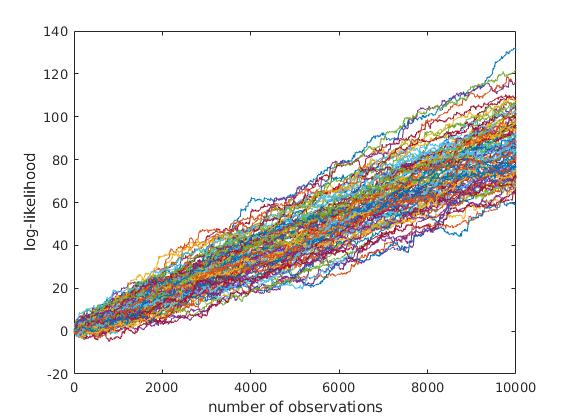
\includegraphics[width=\textwidth/2]{loglikepositiveruns100000_100.jpg}	
		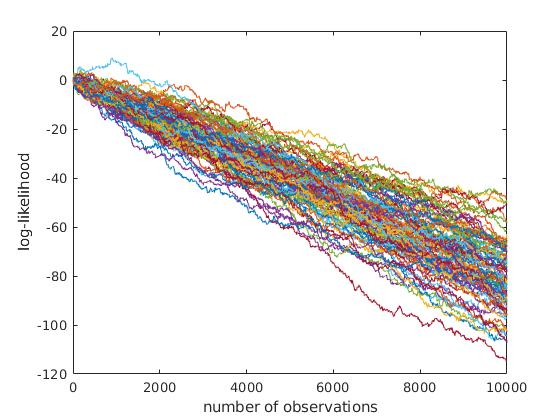
\includegraphics[width=\textwidth/2]{loglikenegativeruns100000_100.jpg}
		\caption{The two images show two log-likelihood plots of sample runs produced by $\pi_1$ and $\pi_2$, respectively.}\label{loglikes}
	\end{figure}
\end{center}
By \Cref{convergenceLn} it follows that $\ln L_n$ converges to $\infty$ and $-\infty$ in the case of words produced by $\pi_1$ and $\pi_2$ respectively. This is affirmed by \Cref{loglikes}. Both log-likelihood plots also appear to follow a particular slope. This suggests that we can distinguish between words produced by $\pi_1$ and $\pi_2$ by tracking the value of $\ln L_n$ to see whether it crosses a lower or upper bound. This is the intuition behind the \emph{Sequential Probability Ratio Test} (SPRT).

%The amount of steps this process takes should also be related to the slope of the slopes.
\end{example}

\section{Sequential Probability Ratio Test}\label{liexpsubsect}

The SPRT runs as follows. We specify two error probabilities $\alpha, \beta > 0$ such that the SPRT gives the result $\pi_2$ from observations produced by $\pi_1$ with probability at most $\alpha$ and similarly the test gives the result $\pi_1$ from observations produced by $\pi_2$ with probability at most $\beta$. We then set $A = \ln \frac{\alpha}{1 - \beta}$ and $B = \ln \frac{1 - \alpha}{\beta}$. The algorithm continues to read observations and computes the value of $\ln L_n$ until $\ln L_n$ leaves the interval $[A,B]$. If $\ln L_n \leq A$ the test result is $\pi_2$ and if $\ln L_n \geq B$ the test result is $\pi_1$. We may express SPRT as a random variable $\SPRT_{\alpha, \beta} : \Sigma^\omega \rightarrow \{\pi_1, \pi_2\}$. We also define the stopping time
\begin{equation*}
N_{\alpha, \beta} = \min \{n \in \NN \mid \ln L_n \not\in [A, B]\}.
\end{equation*}
We have that $N_{\alpha, \beta}$ is monotone decreasing in the sense that for $\alpha' \leq \alpha$ and $\beta' \leq \beta$ we have $N_{\alpha', \beta'} \geq N_{\alpha, \beta}$. When $\pi_1$ and $\pi_2$ are distinguishable $N_{\alpha, \beta}$ is $\PP_{\pi_2}$-almost surely finite by \Cref{convergenceLn}.

\begin{restatable}{theorem}{sprtcorrectness}\label{sprtcorrectness}
Suppose $\pi_1$ and $\pi_2$ are distinguishable. Let $\alpha, \beta$ be inputs to the SPRT. Then by choosing $A = \ln \frac{\alpha}{1 - \beta}$ and $B = \ln \frac{1 - \alpha}{\beta}$, $\PP_{\pi_1} (\SPRT_{\alpha, \beta} = \pi_2) \leq \alpha$ and $\PP_{\pi_2} (\SPRT_{\alpha, \beta} = \pi_1) \leq \beta$.
\end{restatable}


In the following we consider the SPRT with respect to the measure $\PP_{\pi_2}$. This is without loss of generality as there is a dual version of the $\SPRT$, say $\overline{\SPRT}$ with $\overline{L}_n = 1/L_n$ instead of $L_n$, such that $ \overline{\SPRT}_{\beta, \alpha} = \SPRT_{\alpha, \beta}$.

\subsection{Expectation of $N_{\alpha, \beta}$}
Consider the two single state HMMs where $p_1 \neq p_2$. 

\begin{center}
	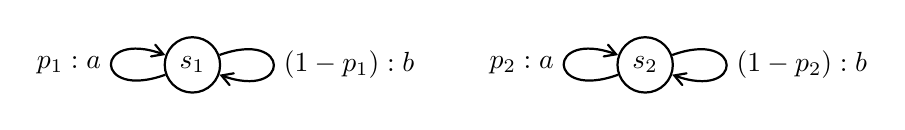
\begin{tikzpicture}[scale=2.3,LMC style]
	\node[state] (s0) at (-1.25,0) {$s_1$};
	\node[state] (s1) at (1.25,0) {$s_2$};
	
	\path[->] (s0) edge [loop,out=200,in=160,looseness=10] node[pos=0.5,left] {$p_1 : a$} (s0);
	\path[->] (s0) edge [loop,out=20,in=340,looseness=10] node[pos=0.5,right] {$(1 - p_1) : b$} (s0);
	\path[->] (s1) edge [loop,out=200,in=160,looseness=10] node[pos=0.5,left] {$p_2 : a$} (s1);
	\path[->] (s1) edge [loop,out=20,in=340,looseness=10] node[pos=0.5,right] {$(1 - p_2) : b$} (s1);
	\end{tikzpicture}
\end{center}

%s_1 and s_2 to match \pi_1 and \pi_2. 

(The Dirac distributions on) $s_1$ and $s_2$ are distinguishable. Further, the increments $\ln L_{n + 1} - \ln L_n$ are i.i.d.\ and $0 > \EE_{s_1}[\ln L_1 - \ln L_0] = p_2 \ln \frac{p_1}{p_2} + (1 - p_2)\ln \frac{1 - p_1}{1 - p_2} =: \ell$. Intuitively as $\ell$ gets more negative, the HMMs become more different.\footnote{In fact, $\ell$ is the \emph{KL-divergence} of the distributions $f_1, f_2$ where $f_i(a) = p_i$ and $f_i(b) = 1 - p_i$ for $i = 1, 2$.} Indeed, Wald~\cite{wald45} shows that the expected stopping time $\EE_{s_2}[N_{\alpha, \beta}]$ and $\ell$ are inversely proportional:
\begin{equation}\label{singletonexptime}
\EE_{s_2}[N_{\alpha, \beta}] = \frac{\beta \ln \frac{1 - \alpha}{\beta} + (1 - \beta) \ln \frac{\alpha}{1 - \beta}}{\ell}.
\end{equation}

This Wald formula cannot hold general (multi-state) HMMs. The increments $\ln L_{n+1} - \ln L_n$ need not be independent and $\EE_{s_1}[\ln L_{n+1} - \ln L_n]$ can be different for different $n$. Further, $| \ln L_{n+1} - \ln L_n |$ can be unbounded --REF-- . 

Nevertheless, in \Cref{loglikes} we observed that $\ln L_n$ appears to decrease linearly (on the $\pi_2$ plot). Indeed we show, in \Cref{liexplimits} below, that the limit $\liexp$ exists $\PP_{\pi_2}$-almost surely. Intuitively it corresponds to the average slope of the log-likelihood plot for $\pi_2$. In the two state case, there is a simple proof of this using the law of large numbers:
\begin{equation*}
\liexp = \lim_{n \rightarrow \infty}\frac1n \sum_{i = 0}^{n - 1} \ln L_{i + 1} - \ln L_i = \EE_{\pi_2} [\ln L_1 - \ln L_0] = \ell \ \ \PP_{\pi_2}\text{-a.s.}
\end{equation*}
The number $\ell$ is called a likelihood exponent, as defined generally in the following definition.
\begin{definition}
A number $\ell$ is a \emph{likelihood exponent} if there are initial distributions $\pi_1$ and $\pi_2$ such that $\PP_{\pi_2}(\liexp = \ell) > 0$.
\end{definition}
\begin{example}\label{multilimitliexp}
There may be multiple likelihood exponents. Consider the following pair of HMMs.

\begin{center}
	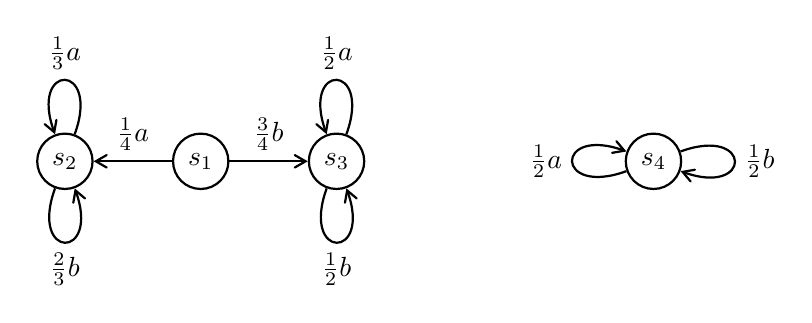
\begin{tikzpicture}[scale=2.3,LMC style]
	\node[state] (s0) at (-1.25,0) {$s_1$};
	\node[state] (s1) at (-2,0) {$s_2$};
	\node[state] (s2) at (-0.5,0) {$s_3$};
	\node[state] (s3) at (1.25,0) {$s_4$};
	
	\path[->] (s0) edge node[pos=0.5,above] {$\frac14 a$} (s1);
	\path[->] (s0) edge node[pos=0.5,above] {$\frac34 b$} (s2);
	
	\path[->] (s1) edge [loop,out=250,in=290,looseness=10] node[pos=0.5,below] {$\frac23 b$} (s1);
	\path[->] (s1) edge [loop,out=70,in=110,looseness=10] node[pos=0.5,above] {$\frac13 a$} (s1);
	
	\path[->] (s2) edge [loop,out=250,in=290,looseness=10] node[pos=0.5,below] {$\frac12 b$} (s2);
	\path[->] (s2) edge [loop,out=70,in=110,looseness=10] node[pos=0.5,above] {$\frac12 a$} (s2);
	
	\path[->] (s3) edge [loop,out=200,in=160,looseness=10] node[pos=0.5,left] {$\frac12 a$} (s3);
	\path[->] (s3) edge [loop,out=20,in=340,looseness=10] node[pos=0.5,right] {$\frac12 b$} (s3);
	\end{tikzpicture}
\end{center}

We observe two different likelihood exponents depending on the first letter produced.  If the first letter is $a$ then $L_1 = \frac12$ and if the first letter is $b$ then $L_1 = \frac32$. If the first letter is $a$ then $\ln L_{n + 1} - \ln L_n$ are i.i.d.\ for $n > 1$ and $\liexp = \frac12 \ln \frac23 +  \frac12 \ln \frac43 = \frac12 \ln \frac89$ like the two state example above. If the first letter is $b$ then $L_n = \frac32$ for all $n > 1$ and $\liexp = 0$. 
\end{example}
We write $\Lambda$ for the set of likelihood exponents in the rest of the paper. In addition, for $\ell \in \Lambda$ we define the event $E_\ell = \{\liexp = \ell\}$. In \Cref{multilimitliexp}, we have $\Lambda = \{\frac12 \ln \frac89, 0\}$. Writing $\ell := \frac12 \ln \frac89$ it follows that $\PP_{s_4}(E_{\ell}) = \PP_{s_4}(E_0) = \frac12$.

\begin{restatable}{theorem}{liexplimits}\label{liexplimits}
The set of likelihood exponents satisfies $\Lambda \subset [-\infty, 0]$ and $|\Lambda| \leq |Q|^2$. Further $\liexp$ exists $\PP_{\pi_2}$-almost surely for any $\pi_1, \pi_2$.
\end{restatable}





We investigate how $\liexp$ influences the performance of the SPRT when $\alpha$ and $\beta$ are small. Intuitively we expect a steeper slope in the likelihood plot (such as in \Cref{loglikes}) to lead to faster termination. In the two state case, Wald's formula \eqref{singletonexptime} becomes 
\begin{equation}\label{asymptoticwaldeq}
\EE_{s_2}[N_{\alpha, \beta}] = \frac{\beta \ln \frac{1 - \alpha}{\beta} + (1 - \beta) \ln \frac{\alpha}{1 - \beta}}{\ell} \sim \frac{\ln \alpha}{\ell} \ (\text{as } \alpha, \beta \rightarrow 0),
\end{equation}
where we use the asymptotic notation $\sim$ defined in the preliminaries. In \Cref{asymptoticwald} below we generalise \Cref{asymptoticwaldeq} to arbitrary HMMs. Indeed a very similar asymptotic identity holds. In the case that $\Lambda = \{\ell\}$ and $\ell \in (-\infty, 0)$ then $\EE_{s_2}[N_{\alpha, \beta}] \sim \frac{\ln \alpha}{\ell}$ as $\alpha, \beta \rightarrow 0$. If $|\Lambda| > 1$ then we condition our expectation on $\liexp$. 

\begin{theorem}[Generalised Wald Formula]\label{asymptoticwald}
Let $\ell$ be a likelihood exponent and let $\pi_1$ and $\pi_2$ be initial distributions. If $\ell \in (-\infty, 0)$ then
\begin{equation*}
\EE_{\pi_2} \Big[ N_{\alpha,\beta} \mid E_{\ell}\Big] \sim \frac{\ln \alpha}{\ell} \ \ (\text{as } \alpha, \beta \rightarrow 0).
\end{equation*}
If $\ell = 0$ then there exist $\alpha, \beta > 0$ such that 
\begin{equation}
\EE_{\pi_2} \Big[ N_{\alpha,\beta} \mid E_\ell\Big] = \infty.
\end{equation}
If $\ell = -\infty$ then 
\begin{equation*}
\sup_{\alpha, \beta}~\EE_{\pi_2} \Big[ N_{\alpha,\beta} \mid E_\ell \Big] < \infty.
\end{equation*}
\end{theorem} 
The theorem above pertains to $\EE_{\pi_2}[N_{\alpha, \beta}]$. In the next subsection we give additional information about the distribution of $N_{\alpha, \beta}$.

\subsection{Distribution of $N_{\alpha, \beta}$}
\subsubsection{Likelihood Exponent $0$}
\begin{example}
We continue with \Cref{multilimitliexp} to illustrate the second case in \Cref{asymptoticwald}. By picking $\alpha = \frac14, \beta = \frac14$ the bounds for the SPRT are $A = \ln \frac13$ and $B = \ln 3$. If the first letter is $b$ then $\ln L_n = \ln \frac32$ for all $n > 1$, thus never crosses the SPRT bounds and $\liexp = 0$. Hence with probability $\frac12$ the SPRT fails to terminate  and $N_{\alpha, \beta} = \infty$. It follows that $\PP_{\pi_2}(E_0) = \frac12$ and $E_{\pi_2}[N_{\alpha, \beta} \mid E_0] = \infty$. Also, $E_{\pi_2}[N_{\alpha, \beta}] = \infty$. 
\end{example}
The second part of \Cref{asymptoticwald} says that the expectation of $N_{\alpha, \beta}$ conditioned under $E_0$ is infinite. The following proposition strengthens this statement. Conditioning under $E_0$, the probability that $N_{\alpha, \beta}$ is infinite converges to $1$ as the errors $\alpha, \beta \rightarrow 0$. Recall that $N_{\alpha, \beta}$ is monotone decreasing. It follows that $\{ N_{\alpha', \beta'} = \infty \} \subset \{ N_{\alpha, \beta} = \infty \}$ if $\alpha' \leq \alpha$ and $\beta' \leq \beta$.
\begin{proposition}\label{probexp0}
The following equalities hold up to $\PP_{\pi_2}$-null sets:
\begin{equation*}
E_0 ~=~ \left\{\lim_{n \rightarrow 0} L_n > 0 \right\} ~=~ \bigcup_{\alpha, \beta} \left\{N_{\alpha, \beta} = \infty\right\}.
\end{equation*}
Thus, $\lim_{\alpha, \beta \rightarrow 0} \PP_{\pi_2}(N_{\alpha, \beta} = \infty) = \PP_{\pi_2}(E_0)$.
\end{proposition}


It follows with \Cref{convergenceLn} that $\pi_1$ and $\pi_2$ are distinguishable if and only if $\PP_{\pi_2}(E_0) = 0$ if and only if $\PP_{\pi_2}(N_{\alpha, \beta} < \infty) = 1$ for all $\alpha, \beta$. 

\subsubsection{Likelihood Exponent $-\infty$}

\begin{example}\label{mortalitywaldex}
Consider now a modification of \Cref{multilimitliexp} where state $s_3$ has the $b$ loop removed.
\begin{center}
	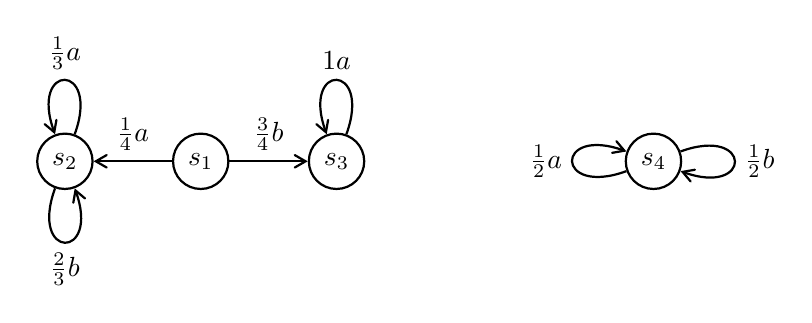
\begin{tikzpicture}[scale=2.3,LMC style]
	\node[state] (s0) at (-1.25,0) {$s_1$};
	\node[state] (s1) at (-2,0) {$s_2$};
	\node[state] (s2) at (-0.5,0) {$s_3$};
	\node[state] (s3) at (1.25,0) {$s_4$};
	
	\path[->] (s0) edge node[pos=0.5,above] {$\frac14 a$} (s1);
	\path[->] (s0) edge node[pos=0.5,above] {$\frac34 b$} (s2);
	
	\path[->] (s1) edge [loop,out=250,in=290,looseness=10] node[pos=0.5,below] {$\frac23 b$} (s1);
	\path[->] (s1) edge [loop,out=70,in=110,looseness=10] node[pos=0.5,above] {$\frac13 a$} (s1);
	
	\path[->] (s2) edge [loop,out=70,in=110,looseness=10] node[pos=0.5,above] {$1 a$} (s2);
	
	\path[->] (s3) edge [loop,out=200,in=160,looseness=10] node[pos=0.5,left] {$\frac12 a$} (s3);
	\path[->] (s3) edge [loop,out=20,in=340,looseness=10] node[pos=0.5,right] {$\frac12 b$} (s3);
	\end{tikzpicture}
\end{center}
The likelihood exponents are $-\infty$ and $\ell := \frac12 \ln \frac89$ so that $\Lambda = \{-\infty, \ell\}$. Also, $\PP_{s_4}(E_{-\infty}) = \PP_{s_4}(E_\ell) =\frac12$. Up to $\PP_{s_4}$-null sets the events $E_{-\infty}$, $b\Sigma^\omega$ and $ba^*b\Sigma^\omega$ are equal. The event $ba^*b\Sigma^\omega$ represents the right chain producing an observation which the left chain cannot produce, causing the SPRT to terminate for any $\alpha, \beta$.
Therefore conditioned on $E_{-\infty}$, the random variable $N_{\alpha, \beta} - 1$ is bounded by a geometric random variable with parameter $\frac12$. Hence $\sup_{\alpha, \beta} \EE_{\pi_2}~ \Big[ N_{\alpha,\beta} \mid E_{-\infty} \Big] \leq 1 + 2$.
\end{example}
We define the stopping time $N_\perp = \min\{n \in \NN \mid L_n = 0\}$. Note that $\sup_{\alpha, \beta}N_{\alpha, \beta} \leq N_\perp$ since $\{L_n = 0\} \subseteq \{L_n \leq \frac{\alpha}{1 - \beta}\}$ for all $\alpha, \beta$. The following proposition states that the reverse inequality also holds.
\begin{proposition}
We have $\sup_{\alpha, \beta} N_{\alpha, \beta} = N_\perp$. Thus, $\lim_{\alpha, \beta \rightarrow 0}\PP_{\pi_2}(N_{\alpha, \beta} < \infty) = \PP_{\pi_2}(E_{-\infty})$.
\end{proposition}
Applying this to \Cref{mortalitywaldex}, we have $\sup_{\alpha, \beta} \EE_{\pi_2}~ \Big[ N_{\alpha,\beta} \mid E_{-\infty}\Big] = 3$.

\subsubsection{Likelihood Exponent in $(-\infty, 0)$}

-- 3 state example where all possibilities are demonstrated on a single graph?



\begin{center}
	\begin{figure}[h]
		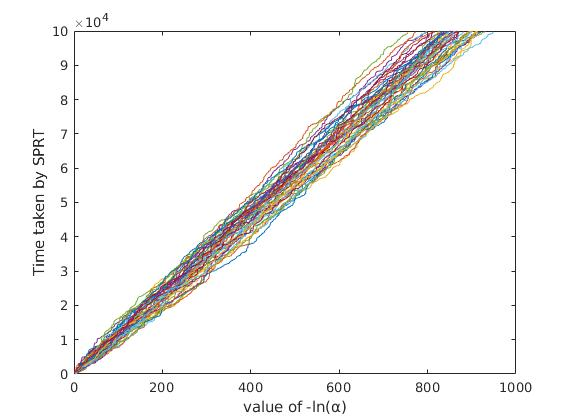
\includegraphics[width=\textwidth]{l100000_i50.jpg}	
		\caption{The image shows the time taken by the SPRT as $-\ln \alpha \rightarrow \infty$.}\label{sprttimevslnalpha}
	\end{figure}
\end{center}

\begin{proposition}\label{liexpmotivation}
Let $\ell \in \Lambda$ and assume $\ell \in (-\infty, 0)$. We have 
\begin{equation*}
\PP_{\pi_2}\left( N_{\alpha,\beta} \sim \frac{\ln \alpha}{\ell} \ \ (\text{as } \alpha, \beta \rightarrow 0) \;\Big\vert\; E_{\ell}\right) ~=~ 1.
\end{equation*}
\end{proposition}

\begin{proof}
Since $\Psimin^n \leq L_n \leq \Psimin^{-n}$ it follows that
\begin{equation*}
N_{\alpha,\beta} \geq \frac{ \min \{ \ln \frac{\alpha}{1 - \beta}, \ln \frac{\beta}{1 - \alpha} \} }{\ln \Psimin}
\end{equation*}
Hence $N_{\alpha, \beta} \rightarrow \infty \ \PP_{\pi_2}$-almost surely as $\alpha, \beta \rightarrow 0$. Consider the case $\ell_k \in (-\infty, 0)$. Let $U_{\alpha,\beta} = \{w \in \Sigma^\omega \mid \ln L_{N_\alpha} \leq \ln \frac{ \alpha}{1 - \beta} \}$. The set $\bigcap_{\alpha, \beta \in (0,1]} U_{\alpha, \beta}^c \subseteq \{L_n \text{ is unbounded}\}$. Hence, $\lim_{\alpha, \beta \rightarrow 0}\1_{U_{\alpha,\beta}} = 1 \ ~\PP_{\pi_2}$-almost surely. Conditioned on $V_k$ it follows that

\begin{equation*}
0 \leq \1_{U_{\alpha, \beta}} \frac{\ln \frac{\alpha}{1 - \beta} - \ln L_{N_{\alpha, \beta}}}{N_\alpha} \leq \1_{U_{\alpha, \beta}}  \frac{\ln L_{N_{\alpha, \beta} - 1}  - \ln L_{N_{\alpha, \beta}}}{N_{\alpha, \beta}}\rightarrow 0 \ \text{ as } \alpha \rightarrow 0.
\end{equation*}
And so 
\begin{equation*}
\lim_{\alpha, \beta \rightarrow 0}\frac{\ln \alpha}{N_{\alpha, \beta}} = \lim_{\alpha \rightarrow 0}\frac{\ln \frac{\alpha}{1-\beta}}{N_{\alpha, \beta}} =\lim_{\alpha \rightarrow 0}\frac{\ln L_{N_{\alpha, \beta}}}{N_{\alpha, \beta}} =\ell_k. 
\end{equation*}
\end{proof}


\section{Computational Aspects}

% distinguishable iff and only if 0 \notin \Lambda
% distinguishable polynomial time
% L_n \rightarrow 0 \pi_2 a.s. iff distinguishable

\begin{proposition}
Whether $0 \in \Lambda$ can be decided in polynomial time. If $0 \in \Lambda$ then $\sup_{\alpha, \beta} \PP_{\pi_2}(N_{\alpha, \beta} = \infty) = \PP_{\pi_2}(E_0)$ can be computed in PSPACE. It is PSPACE-complete to decide whether $\PP_{\pi_2}(E_0) = 1$.
\end{proposition}


\begin{lemma}
Let $S_1, \dots, S_M$ be the bottom connected components of $(\mathcal{S}, P)$. Fix $m \leq M$ and state $(\mu, q) \in S_m$. For the initial distributions $\pi_1 = \mu / \| \mu \|$ and $\pi_2 = e_q$, the likelihood exponent $\liexp$ is $\PP_{\pi_2}$-almost surely a constant. 
\end{lemma}

\begin{lemma}
There is a mapping $\phi : \mathcal{S} \rightarrow \Lambda$ such that for any $\ell \in \Lambda$, the events $\big\{\text{hitting } \phi^{-1}(\ell)\big\}$ and $\{\liexp = \ell\}$ are equal.
\end{lemma}

\begin{lemma}
It is PSPACE-hard to decide whether $\PP_{\pi_2}(E_0) = 1$.
\end{lemma}

\begin{proof}
We reduce from the universality decision problem in NFAs. Let $\mathcal{N} = (Q, \Sigma, \delta, q_0, F)$ be an NFA. Define the HMM $(Q', \Sigma', \Psi)$ where $Q' = Q \cup \{q_\$, q_1\}$ and $\Sigma' = \Sigma \cup \{\$\}$. Then, we may define $\Psi$ as
\begin{equation*}
\Psi(a)_{i,j} = \begin{cases}
\delta(a)_{i,j} / \sum_{k = 1}^{|Q|} \delta(a)_{i,k} & a \in \Sigma,~ i \in Q/F,~ j \in Q \\
\delta(a)_{i,j} / (1 + \sum_{k = 1}^{|Q|} \delta(a)_{i,k}) & a \in \Sigma',~ i \in F,~ j \in Q\\
1 / (1 + \sum_{k = 1}^{|Q|} \delta(a)_{i,k}) & a \in \Sigma',~ i \in F,~ j = s_\$\\
1/|\Sigma'| & a \in \Sigma,~ i = j = q_1 \\
1/|\Sigma'| & a = \$,~ i = q_1,~ j = q_\$ \\
1 & i = j = q_\$\\
0 & \text{else}.\\
\end{cases}
\end{equation*}
Next, let $\pi_1 = e_{q_0}$ and $\pi_2 = e_{q_1}$ be initial distributions. If every word is accepted by $\mathcal{N}$ then for every $w \in (\Sigma)^*$, the event $w\$ \Sigma^\omega = E_0$ since $\lim_{n\rightarrow\infty} L_n > 0$. But up to a $\PP_{\pi_2}$-null set, $\Sigma^* \$ (\Sigma')^\omega = \Sigma^*(\Sigma')^\omega$ which is the set of words that can be generated starting the HMM at $\pi_2$. it follows that $\PP_{\pi_2}(E_0) = 1$. If there is a word $w \in (\Sigma)^*$ which is not final, then the word $w \$$ can be generated with non-zero probability by $\pi_2$ but is a mortal word for $\pi_1$. Hence $\PP_{\pi_2}(E_0) < 1$.
\end{proof}




\begin{proposition}
Deciding whether $-\infty \in \Lambda$ is PSPACE-complete. If $-\infty \in \Lambda$ then $\EE_{\pi_2}[N_\perp | E_{-\infty}] < \infty$ and both $\PP_{\pi_2}(E_{-\infty})$ and $\EE_{\pi_2}[N_\perp | E_{-\infty}]$ are computable in PSPACE. It is PSPACE-complete to decide whether $\PP_{\pi_2}(E_{-\infty}) = 1$.
\end{proposition}

\begin{proof}
Let $\mathcal{S} = \{(\mu, q) \mid \mu \in 2^Q, q \in Q\}$ be a set of states and let 
\begin{equation*}
P_{(\mu_1, i_1), (\mu_2, i_2)} = \sum_{a \in \Sigma}\Psi(a)_{i_1, i_2} \1_{\supp(\mu_1 \Psi(a)) = \mu_2}
\end{equation*}
be a transition matrix. The pair $(\mathcal{S}, P)$ is a Markov chain. Define $\mathcal{K} = \{(\bold{0}, q) \mid q \in Q\}$ and define the initial distribution 
\begin{equation*}
(u_{\pi_1, \pi_2})_{(\mu, i)} = \begin{cases}
(\pi_2)_i & \mu = \supp~\pi_1 \\
0 & \text{else}.
\end{cases}
\end{equation*}
It follows that $\PP_{\pi_2}(N = n) = u_{\pi_1, \pi_2} P^n \chi_{\mathcal{K}}$ since 
\begin{equation*}
\PP_{\pi_2}(N = n) = \PP_{\pi_2}(L_n(w) = 0) \iff \PP_{\pi_2}(\|\pi_1 \Psi(w) \| = 0) \iff \PP_{\pi_2}(\supp (\pi_1 \Psi(w)) = \bold{0}).
\end{equation*}
Therefore $\EE_{\pi_2}[N]$ is equal to the expected hitting time of $\mathcal{K}$ in the Markov chain $(\mathcal{S}, P)$ which has $|Q| \times 2^{|Q|}$ states.

--system can be computed by a PSPACE transducer.
-- Kemeny, Snell book citation   
\end{proof}

\begin{lemma}
Deciding whether $-\infty \in \Lambda$ is PSPACE-hard. 
\end{lemma}
\begin{proof}
Let the matrices $M_1, \dots, M_D \in \{0,1\}^{N \times N}$ be an instance of the mortality problem. If the $i$th row of $\sum_{d = 1}^D M_i$ is a zero row, we may define $M_1', \dots, M_D'$ as the set of matrices $M_1, \dots, M_D$ but with the $i$th row and column removed. $M_1', \dots, M_D'$ is mortal if and only if $M_1, \dots, M_D$ is mortal. 

-- if there is remaining state after the product M' then add an additional letter.

Therefore, without loss of generality, we may assume $\sum_{d = 1}^D M_d$ contains no zero rows. The matrices $\overline{M}_1, \dots, \overline{M}_D$ defined by $\overline{M}_{i,j} = M_{i,j} / \sum_{k = 1}^N M_{i,k}$ are mortal if and only if $M_1, \dots, M_D$ are mortal. Finally, define the HMM $(Q, \Sigma, \Psi)$ where $Q = [N + 1]$, $\Sigma = \{a_1, \dots, a_d\}$ and $\Psi$ is defined in blocks
\begin{equation*}
\Psi(a_i) = \begin{pmatrix}
\overline{M}_i & 0 \\
0 & 1/|\Sigma|
\end{pmatrix}.
\end{equation*}
Let $\pi_1 = (1/N, \dots, 1/N, 0)$ and $\pi_2 = (0, \dots, 0, 1)$. These initial distributions lead to a set of likelihood exponents $\Lambda$ and It follows that $-\infty \in \Lambda$ if and only if $M_1, \dots, M_d$ are mortal.
\end{proof}




Mortality problem



We may assign each end component in $\mathcal{S}$ a symbol denoting which Likelihood exponent is reached. 


\begin{theorem}
The mortality for 
\end{theorem}

proof due to \cite{karasha09}. The hardness result comes from the PSPACE-completeness of mortality problem. 


\begin{corollary}\label{mortality}
$-\infty \in \Lambda$ if and only if there is an $n \leq 2^{|Q|}$ and word $w \in \Sigma^n$ such that $\| \pi_2 \Psi(w) \| > 0$ and $L_n(w) = 0$.
\end{corollary}

\begin{proof}
Clearly if $L_n(w) = 0$ for some word $w \in \Sigma^*$ with $\| \pi_2 \Psi(w) \|$ then $\liexp = -\infty$ with probability atleast $\| \pi_2 \Psi(w) \|$. Suppose then that for all $w \in \Sigma^{2^{|Q|}}$, 
\begin{equation*}
\| \pi_2 \Psi(w) \| > 0 \implies \| \pi_1 \Psi(w) \| > 0
\end{equation*}
then $\| \pi_1 \Psi(w) \| \geq \Psimin^{2^{|Q|}}$. Hence $L_{}$

\end{proof} 

%-=When $\phi \neq \psi$ then $d(s_0, s_1) = 1$, but the expected time for the SPRT is longer if $\lvert \phi - \psi \rvert$ is larger. This corresponds to a more steep slope of sample runs.



\begin{lemma}\label{2016profilethm}
There is a number $c > 0$, computable in polynomial time, such that
\begin{equation*}
\PP_{\pi_2}\Big( L_{2|Q|n} \geq \exp( -\frac{c^2}{36} n ) \Big) \leq 4 \exp\Big( -\frac{c^2}{36} n \Big).
\end{equation*}
\end{lemma}



\begin{proof}
By \Cref{liexpmotivation}, $\lim_{\alpha, \beta \rightarrow 0} \frac{N_{\alpha, \beta}}{\ln \alpha}$ exists $\PP_{\pi_2}( \cdot \mid V_k)$-almost surely. Hence, the convergence is also in $\PP_{\pi_2}( \cdot \mid V_k)$-measure. Therefore, by the Vitali convergence theorem\cite{bog2007} it is sufficient to show that the set of random variables $\{ \frac{N_{\alpha, \beta}}{\ln \alpha} \mid \alpha, \beta \in (0,\frac12) \}$ is uniformly integrable conditioned on $V_k$. In fact, because
\begin{equation}\label{unifintcond}
\lim_{K \rightarrow \infty} \sup_{\alpha, \beta} \EE_{\pi_2} \big[ \frac{N_{\alpha, \beta}}{- \ln \alpha}\1_{\frac{N_{\alpha, \beta}}{-\ln \alpha} \geq - K}\big] \geq \PP_{\pi_2}(V_k) \lim_{M \rightarrow \infty} \sup_{\alpha, \beta} \frac{1}{- \ln \alpha}\EE_{\pi_2} \big[ \frac{N_{\alpha, \beta}}{- \ln \alpha}\1_{\frac{N_{\alpha, \beta}}{-\ln \alpha} \geq - K} \mid V_k \big],
\end{equation}
It is sufficient to check the uniform integrability condition without conditioning on $V_k$.

For fixed $M \geq \frac{144|Q|}{c^2}$, write $m_\alpha = \floor{\frac{- M \ln \alpha}{2|Q|}}$. It follows that $\frac{2|Q|m_\alpha}{\ln \alpha} \leq M$ and $\alpha \geq \exp{-\frac{c^2}{36} m_\alpha}$. Further, $m_\alpha \geq \frac{M \ln 2}{2|Q|} - 1$ The following series of equalities hold
\begin{align*}
 \EE_{\pi_2} \big[ \frac{N_{\alpha, \beta}}{- \ln \alpha} \1_{\frac{N_{\alpha, \beta}}{-\ln \alpha} \geq M}\big] & = \frac{1}{- \ln \alpha} \sum_{n = 0}^\infty \PP_{\pi_2} \big( N_{\alpha, \beta} \1_{N_{\alpha, \beta} \geq 2|Q|m_\alpha}\big] & \leq \frac{2|Q|}{- \ln \alpha}\Big( m_\alpha ~\PP_{\pi_2}(N_{\alpha, \beta} \geq 2|Q|m_\alpha) + \sum_{n = m_\alpha}^\infty \PP_{\pi_2}\big( N_{\alpha, \beta} \geq 2|Q|n\big) > n \Big)\\
& \leq M \PP_{\pi_2}\big( L_{2|Q|m_{\alpha}} \geq \alpha\big) + \frac{2|Q|}{- \ln \alpha} \sum_{n = m_\alpha}^\infty \PP_{\pi_2}\big( L_{2|Q|n} \geq \alpha\big) \\
& \leq M \PP_{\pi_2}\big( L_{2|Q|m_{\alpha}} \geq \exp{-\frac{c^2}{36} m_\alpha}\big) + \frac{2|Q|}{- \ln \alpha} \sum_{n = m_\alpha}^\infty \PP_{\pi_2}\big( L_{2|Q|n} \geq \exp{-\frac{c^2}{36} n}\big) \\
& \leq 4M \exp{-\frac{c^2}{36}m_\alpha}  + \frac{8|Q|}{- \ln \alpha} \sum_{n = m_\alpha}^\infty \exp{-\frac{c^2}{36} n}\\
& \leq 4M \exp{-\frac{c^2}{36}m_\alpha}  + \frac{8|Q|\exp{-\frac{c^2}{36} m_\alpha}}{- \ln \alpha} \frac{1}{1 - \exp{c^2 / 36}}\\
& \leq 4M \exp{-\frac{c^2}{36} \Big(\frac{M \ln 2}{2|Q|} - 1 \Big)}  + \frac{8|Q|\exp \Big( -\frac{c^2}{36} (\frac{M \ln 2}{2|Q|} - 1 ) \Big) }{\ln 2} \frac{1}{1 - \exp{c^2 / 36}}\\
& \rightarrow 0
\end{align*} 
as $K \rightarrow \infty$ where the fourth inequality follows by \Cref{2016profilethm}. Hence, \Cref{unifintcond} must hold. 
\end{proof}
 
\subsection{SPRT for sleep cycles}

\begin{figure}[h]
\begin{center}
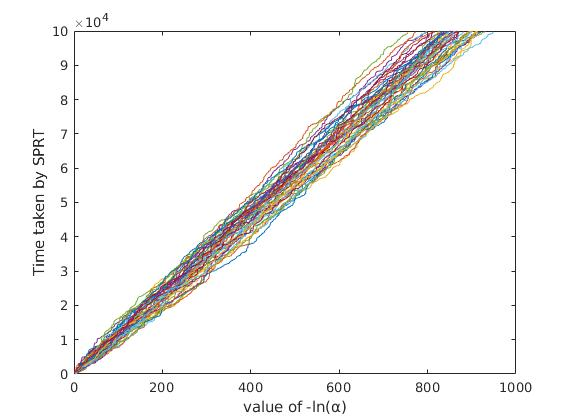
\includegraphics[width=3in]{l100000_i50.jpg}
\caption{$\alpha$ vs $N_\alpha$}\label{stoppingtime}
\end{center}
\end{figure}


\subsection{Deterministic Chains}
A HMM $(Q, \Sigma, \Psi)$ is deterministic if for all $a \in \Sigma$, all rows of $\Psi(a)$ contain exactly one non-zero entry. If $q$ is a starting state, for any word in $w \in \Sigma$ the vector $\delta_q \Psi(w)$ contains at most one non-zero entry. A simple example of a deterministic chain is the following example.

\begin{center}
	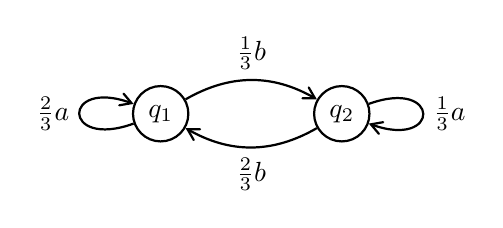
\begin{tikzpicture}[scale=2.3,LMC style]
	\node[state] (s0) at (-0.5,0) {$q_1$};
	\node[state] (s1) at (0.5,0) {$q_2$};
	
	\path[->] (s0) edge [loop,out=200,in=160,looseness=10] node[pos=0.5,left] {$\frac23 a$} (s0);
	\path[->] (s0) edge [out=20,in=170,bend left] node[pos=0.5,above] {$\frac13 b$} (s1);
	\path[->] (s1) edge [out=200,in=340,bend left] node[pos=0.5,below] {$\frac23 b$} (s0);
	\path[->] (s1) edge [loop,out=20,in=340,looseness=10] node[pos=0.5,right] {$\frac13 a$} (s1);
	\end{tikzpicture}.
\end{center}

Suppose two copies of the chain are started from states $q_1$ and $q_2$ respectively, if the chains emit the same word, they will be in opposite states. 
Let the chain started from $q_1$ emit word $aab \in \Sigma^3$. The chain will now be in state $q_2$. Suppose the next letter emitted is $b$. The value of $L_4 = L_3 \times \frac23 / \frac13 = 2 L_3$ and $\ln L_4 = \ln L_3 + \ln 2$. In general deterministic chains have the property that $\ln L_n = R_n + \ln L_{n - 1}$ where $R_n$ is a random variable depending only the transition chosen. In the example above, we can build a Markov chain to characterise the joint distribution of states. We are interested in $\liexp$ with words produced from starting state $q_2$ so the transition probabilities are lifted from the second chain. In the diagram below we also include the value of $R_n$ on each transition.

\begin{center}
	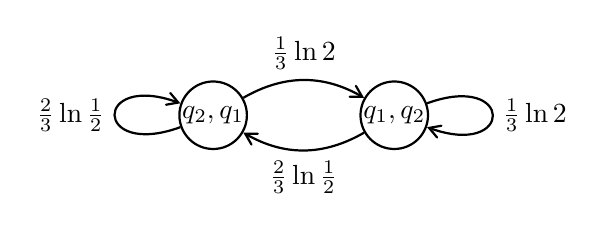
\begin{tikzpicture}[scale=2.3,LMC style]
	\node[state] (s0) at (-0.5,0) {$q_2, q_1$};
	\node[state] (s1) at (0.5,0) {$q_1, q_2$};
	
	\path[->] (s0) edge [loop,out=200,in=160,looseness=10] node[pos=0.5,left] {$\frac23 \ln \frac12$} (s0);
	\path[->] (s0) edge [out=20,in=170,bend left] node[pos=0.5,above] {$\frac13 \ln 2$} (s1);
	\path[->] (s1) edge [out=200,in=340,bend left] node[pos=0.5,below] {$\frac23 \ln \frac12$} (s0);
	\path[->] (s1) edge [loop,out=20,in=340,looseness=10] node[pos=0.5,right] {$\frac13 \ln 2$} (s1);
	\end{tikzpicture}.
\end{center}

The Markov chain has stationary distribution $(\frac23, \frac13)$. By the strong ergodic theorem for Markov chains, $\liexp = \frac13 \ln2 + \frac23 \ln \frac12 = - \frac13 \ln2$. 

In general there may be a finite number of possible limits of $\liexp$. Moreover, these limits may not be rational numbers but expressible as linear combinations of natural logarithms of rational numbers. We say a possible limit of $\liexp$ is $\ln$-symbolically computable if we can compute a set of $2M$ rational numbers where $M \leq |Q|^2$, $\alpha_1, \dots, \alpha_M$ and $\beta_1, \dots, \beta_M$ such that
\begin{equation*}
\liexp = \sum_{l = 1}^M \alpha_m \ln \beta_m.
\end{equation*}

For the general deterministic HMM we simulate the joint state distribution using a Markov chain $M$. This Markov chain has states labelled $(q_i, q_j)$ for $i,j = 1, \dots, |Q|$ and also a special absorbing state $\perp$. The transition probabilities are taken from the outgoing transitions from $q_j$. It may be that a letter produced from $q_j$ cannot be produced from $q_i$ in which case the Markov chain transitions to $\perp$. The full definition is

\begin{align*}
M_{(i, j), (i^*, j^*)} & =\sum_{a \in \Sigma } \Psi(a)_{j, j^*} \delta_{\Psi(a)_{i,i^*} > 0} \\
M_{(i, j), \perp} & = 1 - \sum_{(i^*, j^*) \in [Q \times Q]} M_{(i, j),(i^*, j^*)}  \\
M_{\perp, \perp} & = 1 \\
M_{\perp, (i^*, j^*)} & = 0. \\
\end{align*}

We write $T$ for the set of transitions of $M$. Let $C_0 = \{\perp\}$ and let $C_1, \dots, C_K$ be the remaining bottom connected components of $M$. It follows that the sets $C_0, \dots, C_K$ are disjoint.

\begin{theorem}
Let $(Q, \Sigma, \Psi)$ be a deterministic HMM and let $i_0, j_0$ be the indices of starting states then we may compute a set of symbollic numbers $\{ \lambda_1, \dots, \lambda_K \} \subseteq [-\infty, 0]$ and a probability distribution over these numbers given as $p_1, \dots, p_K$ in $O(|Q|^8)$ time such that, 
\begin{equation*}
\PP_{\delta_{j_0}} \Big( \liexp = \lambda_k \Big) = p_k.
\end{equation*}
for all $k = 1, \dots, K \leq |Q|^2$.
\end{theorem}

\begin{proof}
First assume that the pair $(i_0, j_0)$ is in the bottom connected component $C_k$ with $k \geq 1$ of $M$. Fix $n\in\NN$ then for any $a_1\cdots a_n \in \Sigma^n$, since $\Psi$ is deterministic, there are unique sets of states indexed by $i_1, \dots, i_n$ and $j_1, \dots, j_n$ such that
\begin{equation*}
\frac1n \ln L_n = \frac1n \ln \frac{\Psi(a_1)_{i_0, i_1} \Psi(a_2)_{i_1, i_2} \dots \Psi(a_n)_{i_{n-1}, i_n}}{\Psi(a_1)_{j_0, j_1} \Psi(a_2)_{j_1, j_2} \dots \Psi(a_n)_{j_{n-1}, j_n}} = \frac1n \sum_{m = 1}^n \ln \frac{\Psi(a_m)_{(i_{m - 1}, i_m)}}{\Psi(a_m)_{(j_{m - 1}, j_m)}}.
\end{equation*}
The state pair $(i_m, j_m)$ has the same distribution under $\PP_{\delta_{j_0}}$ as the state distribution of the sub-Markov chain $M$ started from $(i_0 , j_0)$ after $m$ transitions. For each transition in $M$ there is a mapping $l : T  \rightarrow (-\infty, 0]$ given by
\begin{equation*}
l\big( (i,j) \rightarrow (i^*, j^*) \big) = \ln \frac{\Psi(a)_{(i, i^*)}}{\Psi(a)_{(j, j^*)}}.
\end{equation*}
$l$ is well defined because $\Psi$ is deterministic and so $a$ is unique to each transition. Let $\mu^k$ be the unique stationary distribution of the BCC $C_k$. Then by the strong Ergodic theorem, $\liexp$ converges to 
\begin{equation*}
\sum_{(i, j) \rightarrow (i^*, j^*) \in T} \mu^k_{(i, j)} M_{(i,j), (i^*, j^*)} l((i, j) \rightarrow (i^*, j^*)).
\end{equation*}
If the starting state $(i_0, j_0)$ is in $C_0$, then for all possible transitions from $j_0$ in $\Psi$, there are no transitions from $i_0$ and so it follows that $\liexp = -\infty$. Computing the bottom connected components can be done using Tarjan's algorithm in $O(|Q|^2)$ time. Then, computing the stationary distributions $\mu^k$ for $k = 1, \dots, K$ takes $O(|Q|^6)$ time. Therefore, computing the possible $\lambda_1, \dots, \lambda_K$ takes $O(|Q|^6)$ time.

We may write $-\infty = \lambda_0, \dots, \lambda_K$ for the possible limits of $\frac1n \ln L_n$ starting in $C_0, \dots, C_K$ respectively. We write $C^{-1}(\lambda_k)$ for the union of bottom connected components associated with the likelihood exponent $\lambda_k$. In general, for starting states $(i,j)$, $\liexp = \lambda_k$ when the Markov chain $M$ hits any of the states in $C^{-1}(\lambda_k)$. Therefore computing $p_1, \dots, p_k$ is equivalent to computing a hitting probability which can be done in $O(|Q|^6)$ because $M$ has dimension at most $|Q|^2$. This makes the whole algorithm $O(|Q|^8)$ since $K \leq |Q|^2$.
\end{proof}

\subsection{Non-Deterministic Chains}

- show that it's atleast PSPACE hard to approximate and computing them is as hard as computing lyapunov exponents (known to be a hard problem).





By introducing non-determinism, the likelihood ratio can no longer be split into a simple product of random variables depending only on the transitions in a Markov chain. It follows that we may not use the Strong ergodic theorem for Markov chains to show convergence of $\liexp$. We instead prove convergence using work by Protasov. The following theorem is proven in the appendix.

We say an HMM $(Q, \Sigma, \Psi)$ is strongly connected if the Markov chain $\sum_{a \in \Sigma} \Psi(a)$ is strongly connected. An HMM is \emph{lossy} if $\sum_{a \in \Sigma} \Psi(a)$ is sub-stochastic.

\begin{restatable}{theorem}{nondetermconv}\label{nondetermconv}
Let $(Q, \Sigma, \Psi)$ be an HMM and let $\pi_1, \pi_2$ be initial distributions. Then $\liexp$ converges $\pi_2$-almost surely to at most $|Q|^2$ values in the set $[-\infty, 0]$.

We may compute in polynomial time a set of strongly connected lossy HMMs $(Q_k, \Sigma, \Psi_k)$ and pairs of initial states $(q_k, r_k)$ with corresponding likelihood ratios $L^k_n$ such that $\liexp^k$ takes a single value $\PP_{\delta_{r_k}}$-almost surely. Moreover
\begin{equation*}
\liexp \in \{\liexp^k \mid k = 1, \dots, K\}.
\end{equation*}
\end{restatable} 

There is no known algorithm for computing each limit $\liexp^k$. Moreover, even if we know the values of $\liexp^k$, we show that computing the distribution of $\liexp$ over the possible limits $\{\liexp^k \mid k = 1, \dots, K\}$ is PSPACE-complete. We therefore consider consider a series of problems leading up to the final result.

The starting point is language inclusion for \emph{non-deterministic finite automata} (NFA). An NFA is a quintuple $(Q,\Sigma ,\Delta ,q_0,F)$ such that
The starting point is language inclusion for \emph{non-deterministic finite automata} (NFA). An NFA is a quintuple $(Q,\Sigma ,\Delta ,q_0,F)$ such that
\begin{itemize}
\item a finite set of states $Q$.
\item a finite set of input symbols $\Sigma$.
\item a transition function $\Delta : Q \times \Sigma \rightarrow \mathscr{P}(Q)$.
\item an initial state $q_0$
\item a set of final states $F \subseteq Q$.
\end{itemize}
The language accepted by $M$, $L(M)$ is the set of $a_1\cdots a_n \in \Sigma^n$ such that there exists a sequence of states $q_1, \dots, q_n$ such that $q_i \in \Delta (q_{i - 1}, a_i)$ for $i = 1, \dots, n$ and $q_n \in F$.

\paragraph*{NFA language inclusion\\}
Let $M_1$ and $M_2$ be two NFAs with the same set of input symbols. Decide whether $L(M_1) \subseteq L(M_2)$.

\paragraph*{The Likelihood Mortality Problem\\}
Given an HMM $(Q, \Sigma, \Psi)$ and initial distributions $\pi_1, \pi_2$ such that $\liexp$ converges to a single value, decide whether $\liexp = -\infty$ $\PP_{\pi_2}$-almost surely.

\paragraph*{The Likelihood Exponent $\epsilon$-approximation problem\\}
Fix $\epsilon > 0$ and. Given a strongly connected non-mortal HMM and two initial distributions $\pi_1, \pi_2$ compute a rational number (or $-\infty$) labelled $\Lambda^* \in [-\infty, 0]$ such that
\begin{equation*}
\big\lvert \liexp - \Lambda^* \big\rvert \leq \epsilon \quad \PP_{\pi_2}\text{-a.s.}
\end{equation*}

\paragraph*{The Likelihood Exponent comparison problem\\}
Let $(Q_1, \Sigma, \Psi_1)$ and $(Q_2, \Sigma, \Psi_2)$ be strongly connected HMMs with likelihood exponents $\liexp^1$ and $\liexp^2$ respectively. Decide whether $\liexp^1 < \liexp^2$.

\paragraph*{The Likelihood Exponent distribution problem\\}
By \Cref{nondetermconv} we know the values of likelihood exponent candidates $\liexp \in \{\liexp^k \mid k = 1, \dots, K\}$. Compute a set of numbers $p_1, \dots, p_K$ such that 
\begin{equation*}
\PP_{\pi_2}\Big(\liexp = \liexp^k \Big) = p_k
\end{equation*}
for all $k = 1, \dots, K$.

The following theorem is from \cite{kupvar98}.
\begin{theorem}
NFA language inclusion is PSPACE-complete.
\end{theorem}

We show that this problem is equivalent to the \emph{Mortality problem} in the following lemma.

\begin{lemma}\label{mortalpspace}
The Likelihood Mortality problem is PSPACE-complete. 
\end{lemma}

For two matrices $A, B \in \RR^{N \times N}$, Let the matrix $A \bigoplus B \in \RR^{2N \times 2N}$ be defined in blocks as

\begin{equation*}
A \bigoplus B = \begin{pmatrix}
A & 0 \\
0 & B \\
\end{pmatrix}.
\end{equation*}


\begin{proof}[Proof of \Cref{mortalpspace}]
We show that the problem is hard even for a subset of HMMs and initial distributions. Let $(Q, \Sigma, \Psi)$ be an HMM and consider a new HMM
$(Q \cup \{q^*\}, \Sigma, \Psi \bigoplus f)$ where $q^*$ is an additional state and $f : \Sigma \rightarrow [0,1]$ is defined by $f(a) = \frac{1}{|\Sigma|}$. Consider the initial distributions $(1, 1, \dots, 1, 0) \in [0,1]^{|Q| + 1}$ and $(0, \dots, 0, 1) \in [0,1]^{|Q| + 1}$ then mortality is PSPACE-hard even for these HMMs and initial distributions. Proof of this is due to \cite{karasha09}.

To show completeness, consider an instance of the Likelihood mortality problem $(Q, \Sigma, \Psi)$ with initial distributions $\pi_1, \pi_2$. We construct two NFAs $M_i = (Q \cup \{q_0^i\}, \Sigma, \Delta, q_0^i, Q)$ for $i = 1, 2$ where $\Delta(q_0^i, a) = \supp \pi_i$ for all $a \in \Sigma$. If $L(M_1) \not\subseteq L(M_2)$ then there is a word $w \in \Sigma^n$ such that $\pi_2 \Psi(w) \1 > 0$ but $\pi_1 \Psi(w) \1 = 0$ hence $\liexp = -\infty$. Now assume $L(M_1) \subseteq L(M_2)$. Let $A_n = \{ w \in \Sigma^n \mid \pi_2 \Psi(w) \1^T > 0 \}$ and $\PP_{\pi_2}(A_n \Sigma^\omega) = 1$ for all $n \in \NN$. It follows by language inclusion that a word $w \in A_n$ also has the property that $\pi_1 \Psi(w) \1^T > 0$ hence $\pi_1 \Psi(w) \1^T > \Psi_{\text{min}}^n$ hence $\liexp \geq \Psi_{\text{min}} > -\infty$.
\end{proof}

The proof of the following propositions have been omitted for now.

\begin{proposition}
The likelihood exponent $\epsilon$-approximation problem is PSPACE-hard. 
\end{proposition}

\begin{proof}
consider an instance of the $0-1$ matrix mortality problem. 
\end{proof}

\begin{proposition}
The likelihood exponent comparison problem is PSPACE-hard. 
\end{proposition}

\begin{proposition}
The likelihood exponent distribution problem is PSPACE-hard. 
\end{proposition}





\bibliography{lyapunovhmm}

\appendix

\convergenceLn*

\begin{proof}
By proposition 6 in \cite{kief14} the limit $L_n$ exists $\PP_{\pi_2}$-a.s. and the following equalities hold. 
\begin{align*}
1 - d(\pi_1, \pi_2) & = \lim_{n \rightarrow \infty} \sum_{w \in \Sigma^n} \| \pi_1 \Psi(w) \| \land \| \pi_2 \Psi(w) \| && \text{Theorem 7 of \cite{kief14}}\\
& = \lim_{n \rightarrow \infty} \sum_{w \in \Sigma^n} (L_n(w) \land 1 ) \| \pi_2 \Psi(w)\| \\
& = \lim_{n \rightarrow \infty} \EE_{\pi_2} \big[ L_n \land 1  \big] \\
& = \EE_{\pi_2} \big[ \lim_{n \rightarrow \infty}  L_n \land 1  \big] && \text{because } 0 \leq L_n(w) \land 1 \leq 1.
\end{align*}
Then, $\lim_{n \rightarrow \infty}  L_n \land 1 = 0 \iff \lim_{n \rightarrow \infty}  L_n = 0$.
\end{proof}


\section{SPRT Correctness}

\sprtcorrectness*

\begin{proof}
We wish to control the probabilities $\PP_{\pi_2}\big( L_N > B\big)$ and $\PP_{\pi_1}\big( L_N < A\big)$ by choosing suitable values of $A$ and $B$. Let $W_n^1 = \{ w \in \Sigma^\omega \mid  A \leq L_m(w) \leq B ~\forall m < n, L_n < A\}$ then

\begin{align*}
\PP_{\pi_1}\big( L_N < A \big) & = \sum_{n = 1}^\infty \PP_{\pi_1}\big( W_n^1 \big) = \sum_{n = 1}^\infty \sum_{w \in W_n^1} \pi_1 \Psi(w) \1^T = \sum_{n = 1}^\infty \sum_{w \in W_n^1} L_n(w) \pi_2 \Psi(w) \1^T \\
& \leq A \sum_{n = 1}^\infty  \sum_{w \in W_n^1} \pi_2 \Psi(w) \1^T = A \sum_{n = 1}^\infty  \PP_{\pi_2}\big( W_n^1 \big) = A \PP_{\pi_2}\big( L_N < A \big). \\
\end{align*}

Similarly, we may derive $\PP_{\pi_2}\big( L_N > b \big) \geq \frac{1}{b} \PP_{\pi_1}\big( L_N > b\big)$ so it follows that

\begin{align*}
A & \geq \frac{\PP_{\pi_1}\big(  L_N < A\big)}{\PP_{\pi_2}\big(  L_N < A\big)} = \frac{\PP_{\pi_1}\big(  L_N < A\big)}{1 - \PP_{\pi_2}\big(  L_N > B\big)} \\
B & \leq \frac{\PP_{\pi_1}\big(  L_N > B\big)}{\PP_{\pi_2}\big(  L_{N} > B\big)} = \frac{1 - \PP_{\pi_1}\big( L_N < A\big)}{\PP_{\pi_2}\big(  L_N > B\big)}\\
\end{align*}
to guarantee the error bounds $\alpha = \PP_{\pi_1}\big( L_{n^*} < A\big)$ and $\beta = \PP_{\pi_2}\big( L_{n^*} > B\big)$.
\end{proof}

\section{Proof of Lyapunov Exponent Convergence}

\subsection{Proof of \Cref{nondetermconv}}

The proof of \Cref{nondetermconv} relies on related work in a subset of Ergodic Theory called \emph{Lyapunov exponents}. The main papers are by Protasov \cite{prot13} and Osedelets \cite{ose68}. We first must define a similar object to a observation density matrix. A \emph{random matrix product} is a triple $(Q, \Sigma, \Phi)$ where $Q$ is a set of states, $\Sigma$ is a set of letters and $\Phi : \Sigma \rightarrow [0,1]^{|Q| \times |Q|}$ is a non-negative matrix valued function. We may extend $\Phi$ to $\Sigma^*$ in the same way as an observation density matrix. we use the shorthand $\Phi_n : \Sigma^n \rightarrow [0,1]^{|Q| \times |Q|}$ for $\Phi$ restricted to $\Sigma^n$. $(Q, \Sigma, \Phi)$ is strongly connected if for all $i,j \in [Q]$ there exists a  $w \in \Sigma^*$ such that $\Phi(w)_{i,j} > 0$. $(Q, \Sigma, \Phi)$ is mortal if there exists a $w \in \Sigma^*$ such that $\Phi(w) = 0$. The main theorem by Protasov is stated below. 

\begin{theorem}\textsc{\textbf{Protasov's Theorem}}\label{protstheorem}
Let $(Q, \Sigma, \Phi)$ be a strongly connected random matrix product, let $\PPind$ be an i.i.d probability measure on $\Sigma^\omega$ and let $\pi$ be an initial distribution. If $(Q, \Sigma, \Phi)$ is mortal, then $\lim_{n \rightarrow \infty} \frac1n \ln \pi \Phi_n \1^T = -\infty \quad \PPind$-a.s. otherwise there is a $\lambda \in (-\infty, 0]$ such that $\lim_{n \rightarrow \infty} \frac1n \ln \pi \Phi_n \1^T = \lambda \quad \PPind$-a.s.
\end{theorem}

The technique we use to prove \Cref{nondetermconv} involves producing an i.i.d measure $\PPind$ and random matrix product $(Q \times Q, \Sigma, \Phi)$ such that for all $n \in \NN$ and initial distributions $\pi$,
\begin{equation*}
\PPind\Big( \frac1n \ln \pi \Phi_n \1^T \in A \Big) = \PP_{\pi_2}\Big( \frac1n \ln \pi \Psi_n \1^T \in A\Big).
\end{equation*}

Since $\liexp = \lim_{n \rightarrow \infty} \frac1n \ln \pi_1 \Psi_n \1^T - \lim_{n \rightarrow \infty} \frac1n \ln \pi_2 \Psi_n \1^T$ such a random matrix product would imply convergence of $\liexp$ due to Protasov's theorem.

When the probability space on infinite words is derived from a general HMM, the probability of a particular letter being produced at a specific position in the infinite word depends on the state the producing HMM is in. In the constructed random matrix product, the current state of the producing HMM as started from $\pi_2$ is incorporated into the state space of the HMM started from $\pi_1$. 

To accomplish this, we simulate transitions in the producing HMM (the chain started from $\pi_2$) by sampling a uniform random number in the interval $[0,1)$. At each state, we may partition $[0,1)$ so that each sub-interval corresponds to specific transition and the size of the sub-interval corresponds to the probability of said transition. The union over all states of these partitions has a minimal finite $\sigma$-algebra. The atoms of this $\sigma$-algebra are also a partition of $[0,1)$ and so we may sample them independently at random with probabilities according to their size. The transformation on a simple example is demonstrated in the diagram below. On the left is the original HMM. On the right is a single state HMM representing $\PPind$. For example, with probability $\frac16$, it produces the label $[\frac13, \frac12)$ which corresponds to the $b$ transition in $s_0$ or the $a$ transition in $s_1$.

\begin{center}
	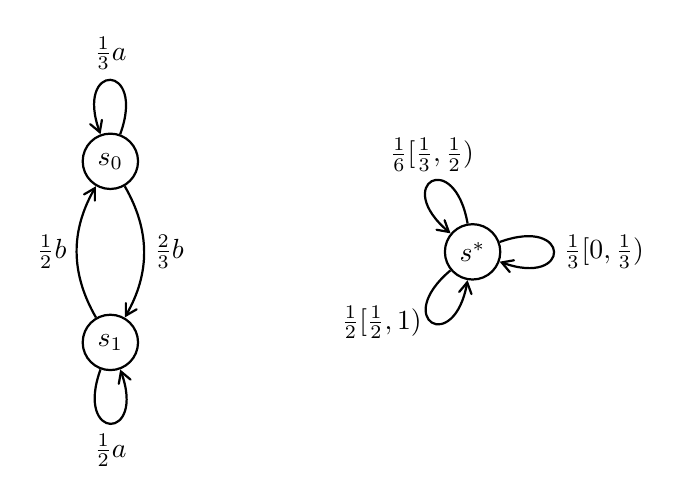
\begin{tikzpicture}[scale=2.3,LMC style]
	\node[state] (s0) at (-1,1) {$s_0$};
	\node[state] (s1) at (-1,0) {$s_1$};
	\node[state] (s2) at (1,0.5) {$s^*$};

	
	\path[->] (s0) edge [loop,out=70,in=110,looseness=10] node[pos=0.5,above] {$\frac13 a$} (s0);
	\path[->] (s1) edge [loop,out=250,in=290,looseness=10] node[pos=0.5,below] {$\frac12 a$} (s1);
	\path[->] (s1) edge[bend left] node[left,pos=0.5] {$\frac12 b$} (s0);
	\path[->] (s0) edge[bend left] node[right,pos=0.5] {$\frac23 b$} (s1);
	
	\path[->] (s2) edge [loop,out=20,in=340,looseness=10] node[pos=0.5,right] {$\frac13 [0,\frac13)$} (s2);
	\path[->] (s2) edge [loop,out=100,in=140,looseness=10] node[pos=0.5,above] {$\frac16 [\frac13, \frac12)$} (s2);
	\path[->] (s2) edge [loop,out=220,in=260,looseness=10] node[pos=0.5,left] {$\frac12 [\frac12,1)$} (s2);
	\end{tikzpicture}
\end{center}

We now construct the random matrix product $(Q \times Q, \Sigma, \Phi)$ which can also be represented by a state transition system (but without any stochastic properties). In our example, $(Q \times Q, \Sigma, \Phi)$ consists of two strongly connected components. Each state is labelled with a left and right component state corresponding to the current states of the HMM started from $\pi_1$ and $\pi_2$ respectively. The transition weights are taken from the transitions in $\pi_1$ and the transition letters are taken from the transitions in $\pi_2$ because this random matrix product simulates $\frac1n \ln \pi_1 \Psi_n \1^T$ under the probability measure $\PP_{\pi_2}$.

\begin{center}
	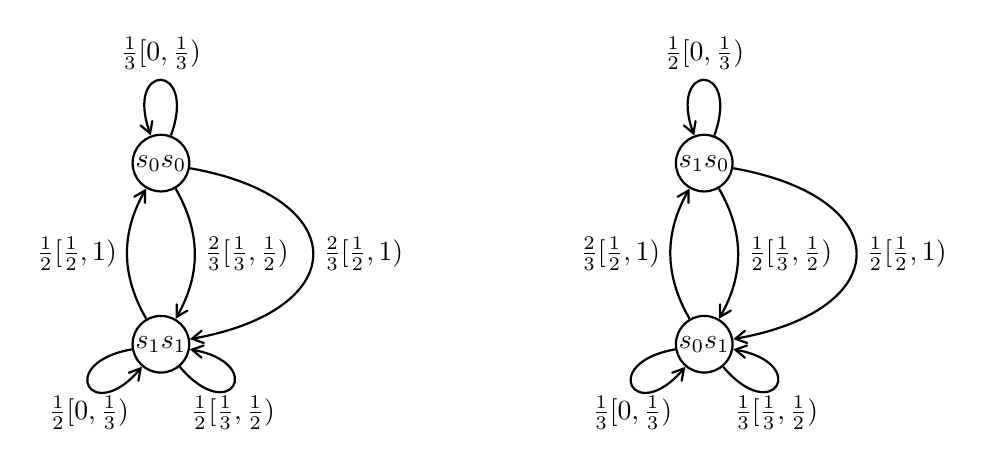
\begin{tikzpicture}[scale=2.3,LMC style]
	\node[state] (s0s0) at (-1.5,1) {$s_0 s_0$};
	\node[state] (s1s1) at (-1.5,0) {$s_1 s_1$};
	\node[state] (s1s0) at (1.5,1) {$s_1 s_0$};
	\node[state] (s0s1) at (1.5,0) {$s_0 s_1$};
	
	\path[->] (s0s0) edge [loop,out=70,in=110,looseness=10] node[pos=0.5,above] {$\frac13 [0,\frac13)$} (s0s0);
	\path[->] (s0s0) edge[bend left] node[right,pos=0.5] {$\frac23 [\frac13,\frac12)$} (s1s1);
	\path[->] (s0s0) edge[bend left, out=80, in=100, looseness = 2.5] node[right,pos=0.5] {$\frac23 [\frac12, 1)$} (s1s1);	
	
	 \path[->] (s1s1) edge[bend left] node[left,pos=0.5] {$\frac12 [\frac12, 1)$} (s0s0);
	\path[->] (s1s1) edge [loop,out=190,in=230,looseness=10] node[pos=0.5,below] {$\frac12 [0,\frac13)$} (s1s1);
	\path[->] (s1s1) edge [loop,out=310,in=350,looseness=10] node[pos=0.5,below] {$\frac12 [\frac13,\frac12)$} (s1s1);
	
	
	\path[->] (s1s0) edge [loop,out=70,in=110,looseness=10] node[pos=0.5,above] {$\frac12 [0,\frac13)$} (s1s0);
	\path[->] (s1s0) edge[bend left] node[right,pos=0.5] {$\frac12 [\frac13,\frac12)$} (s0s1);
	\path[->] (s1s0) edge[bend left, out=80, in=100, looseness = 2.5] node[right,pos=0.5] {$\frac12 [\frac12, 1)$} (s0s1);	
	
	\path[->] (s0s1) edge [loop,out=190,in=230,looseness=10] node[pos=0.5,below] {$\frac13 [0,\frac13)$} (s0s1);
	\path[->] (s0s1) edge [loop,out=310,in=350,looseness=10] node[pos=0.5,below] {$\frac13 [\frac13,\frac12)$} (s0s1);
	\path[->] (s0s1) edge[bend left] node[left,pos=0.5] {$\frac23 [\frac12, 1)$} (s1s0);
		
	\end{tikzpicture}
\end{center}

\paragraph{Random Matrix Product Construction\\}
Consider the HMM $(Q, \Sigma, \Psi)$ with finite alphabet $\Sigma$. Since for each $i \in [Q]$, $\sum_{a \in \Sigma} \sum_{j = 1}^{|Q|} \Psi(a)_{i,j} = 1$ it follows that we may define a function $\rho_i : [0,1) \rightarrow Q \times \Sigma$ such that for all $i \in [Q]$, $\MLeb(\rho_i^{-1}\{(j, a)\}) = \Psi(a)_{i,j}$. Consider the minimal $\sigma$-algebra $\sigma\{\rho_i^{-1}\{(j, a)\} \mid i,j \in [Q], a \in \Sigma\}$ which is finite and has a set of atomic elements $P$ of at most $|Q|^2|\Sigma|$ elements. $P$ is also a partition of $[0,1)$. Let $p \in P$ then $\rho_i(x)$ is constant for all $x \in p$ so we may overload the notation and consider the function $\rho_i : P \rightarrow Q \times \Sigma$. 

We will describe the one-state chain $(\{1\}, P, \Psi_P)$ as the \emph{singleton generator} for $\Psi$ where $\Psi_P(p) = \MLeb(p)$. Given an initial distribution $\pi$ for $(Q, \Sigma, \Psi)$, a word generated by its singleton generator uniquely defines a path of states and letters. Let $\PPind$ be the measure on the set of infinite words $P^\omega$ generated by this HMM.

In order to incorporate the state space of the producing HMM into the state space of the chain started from $\pi_1$, we define two functions $l : Q \times \Sigma \rightarrow Q$ and $r : Q \times \Sigma \rightarrow \Sigma$ where $l(q,a) = q$ and $r(q,a) = a$. We then define the matrix valued function $\Phi : P \rightarrow [0,1]^{(Q \times Q) \times (Q \times Q)}$ as 

\[\Phi(p)_{(i_1,j_1),(i_2,j_2)} = \begin{cases} 
\Psi(r \circ \rho_{j_1}(p) )_{i_1, i_2} & l \circ \rho_{j_1}(p) = j_2 \\
0 & \text{else}. \\
\end{cases}\]

\begin{proposition}\label{existenceoflims}
Consider the HMM $(Q, \Sigma, \Psi)$ with initial distributions $\pi_1$ and $\pi_2$ then for any measurable set $A \in [-\infty, 0]$ and for all $n \in \NN$
\begin{equation*}
\PP_{\pi_2}\Big( \frac1n \ln L_n \in A\Big) = \PPind\Big( \frac1n \ln \frac{\pi_1 \times \pi_2 \Phi_n \1}{\pi_2 \times \pi_2 \Phi_n \1} \in A \Big).
\end{equation*}
\end{proposition}

\begin{proof}
We can extend $\rho_i$ to $\rho_i : P^n \rightarrow (Q \times \Sigma)^n$ by iteratively defining $\rho_i(ua) = \rho_i(u) \rho_{l(\rho_i(u))}(a)$. Let  $i_0, j_0 \in [Q]$ be initial states, It follows that for a word $u_1 \dots u_n \in \{\rho_{j_0}(u_1 \dots u_n) = (j_1, a_1), \dots, (j_n, a_n)\}$,

\begin{align*}
\| e_{i_0}^T e_{j_0} \Phi(u) \| & = \sum_{(i_1, \dots, i_n) \in [Q]^n} \Phi(u_1)_{(i_0, j_0),(i_1,j_1)} \dots \Phi(u_n)_{(i_{n - 1}, j_{n - 1}),(i_n,j_n)}\\
& = \sum_{(i_1, \dots, i_n) \in [Q]^n} \Psi(a_1)_{i_0, i_1} \dots \Psi(a_n)_{i_{n - 1}, i_n}\\
& = \| e_{i_0} \Psi(a_1 \dots a_n) \|.
\end{align*}
It follows that for any initial distributions $\pi_1, \pi_2$, $\| \pi_1^T \pi_2 \Psi^*(u) \| = \| \pi_1 \Psi(a_1 \dots a_n) \|$. Then considering the word $a_1, \dots, a_n$, 

\begin{align*}
\PP_{\pi_2}(a_1 \dots a_n) & =\|\pi_2\Psi(a_1 \dots a_n)\| \\
& = \sum_{j_1, \dots, j_n \in [Q]^n}\|\pi_2\Psi(a_1)_{\pi_2, j_1} \dots \Psi(a_n)_{j_{n - 1}, j_n}\|\\
& = \sum_{u_1, \dots, u_n \in \{\rho_{\pi_2}(u_1, \dots, u_n) = (j_1, a_1), \dots, (j_n, a_n)\}} \Psi_P(u_1 \dots u_n)\\
& = \PP_{\text{ind}}(l \circ \rho_{\pi_2}(u_1 \dots u_n) = a_1 \dots a_n)
\end{align*}
\end{proof}


Consider the bottom connected components $C_1, \dots, C_k \subseteq Q \times Q$ of the Markov chain defined by $\sum_{p \in P} \Phi(p)$ and let $d : Q \times Q \rightarrow Q \times Q$ be defined as $d(s_1, s_2) = (s_2, s_2)$. The following lemmas give the $|Q|^2$ bound in \Cref{nondetermconv}.

\begin{lemma}\label{Qboundfordenominator}
Let $s$ be a starting state for an HMM $(Q, \Sigma, \Psi)$. Then $\lim_{n \rightarrow \infty} \frac1n \ln \|  (s, s) \Psi_n^* \|$ takes at most $|Q|$ values.
\end{lemma}

\begin{proof}
Let $P_1, \dots, P_K$ be the irreducible components of $\Phi$. Consider states $(s_1, s_2), (r_1, r_2) \in Q \times Q$. If there is a path from $(s_1, s_2)$ to $(r_1, r_2)$ then there is also a path from $(s_2, s_2)$ to $(r_2, r_2)$. Therefore for any end component $P_i$ it follows that the image $d(P_i) \subseteq P_j$ for some end component $P_j$ and so we may define a function $\rho : \{ P_1, \dots, P_K \} \rightarrow \{ P_1, \dots, P_K \}$ such that $\rho(P_i) = P_j$. Suppose $P_i, P_j$ have Lyapunov exponents $\lambda_i$ and $\lambda_j$ respectively. Let $\pi_1$ and $\pi_2$ be initial distributions such that the support of $\pi_1$ is in $P_i$ and the support of $\pi_2$ is in $P_j$ then the likelihood ratio $L_n = \frac{\| \pi_1 \Psi_n \|}{\| \pi_2 \Psi_n \|}$ converges to a limit in the set $[0,\infty)$ with respect to the measure $\PP_{\pi_2}$, the same limit as $\frac{\| (\pi_1, \pi_2) \Psi_n^* \|}{\| (\pi_2, \pi_2) \Psi_n^* \|}$ with respect to $\PP_\text{ind}$. Since both $\frac{1}{n} \ln \| (\pi_1, \pi_2) \Psi_n^* \|$ and $\frac{1}{n} \ln \| (\pi_2, \pi_2) \Psi_n^* \|$ converge almost surely in the set $[-\infty, 0]$ to $\lambda_i$ and $\lambda_j$ respectively, $\frac{1}{n} \ln \frac{\| \pi_1 \Psi_n \|}{\| \pi_2 \Psi_n \|}$ converges in $[-\infty, 0]$ with respect to $\PP_{\pi_2}$. Therefore $\lambda_i \leq \lambda_j$.
Now consider $\lim_{n \rightarrow \infty} \frac1n \ln \|  (s, s) \Psi_n^* \|$ whose possible limits is bounded by $|Q|^2$. Suppose for some word $w \in P^n$ the support of $(s, s) \Psi_n^*$ intersects an irreducible component $P_i$. Then it must also intersect $P_j$. Since $\lambda_i \leq \lambda_j$ it follows that $\lim_{n \rightarrow \infty} \frac1n \ln \|  (s, s) \Psi_n^* \| \geq \lambda_j$. Since the image $\rho \{P_1, \dots, P_K \} \leq |Q|$ it follows that $\lim_{n \rightarrow \infty} \frac1n \ln \|  (s, s) \Psi_n^* \|$ takes at most $|Q|$ values.
\end{proof}

\begin{lemma}\label{qsquaredboundlike}
Consider an HMM $(Q, \Sigma, \Psi)$. Let $\Epsilon : [0,1]^{|Q|} \times [0,1]^{|Q|} \rightarrow [\infty, 0]$ be a parametrised random variable on $\Sigma^\omega$ defined by $\Epsilon(\pi_1, \pi_2) = \lim_{n \rightarrow \infty} \frac1n \ln \frac{\| \pi_1 \Psi(w) \|}{\|\pi_2 \Psi(w) \|}$. Then $|\{\Epsilon(\pi_1, \pi_2) \mid \pi_1, \pi_2 \in [0,1]^{|Q|}\} | \leq |Q|^2$ with respect to the measure $\PP_{\pi_2}$.
\end{lemma}

\begin{proof}
First consider the case of dirac distributions $\pi_1 = \delta_r$ and $\pi_2 = \delta_s$. We may instead consider a bound on
\begin{equation*}
\lim_{n \rightarrow \infty} \frac{1}{n} \ln \frac{\| (\delta_r, \delta_s) \Psi_n^* \|}{\| (\delta_s, \delta_s) \Psi_n^* \|} = \lim_{n \rightarrow \infty} \frac1n \ln \| (\delta_r, \delta_s) \Psi_n^*\| - \lim_{n \rightarrow \infty} \frac1n \ln \| (\delta_s, \delta_s) \Psi_n^*\|
\end{equation*}
with respect to the $\PP_\text{ind}$ measure. Let $C_1, \dots, C_K$ be the irreducible lethal components of $\Phi$. For $L \leq K$ without loss of generality suppose $C_1, \dots, C_L$ be the irreducible components that are also end components containing diagonal entries. Let $R_1, \dots, R_L \subseteq Q$ be disjoint and have the property that for all $q \in R_i$, $(q, q) \in C_i$. 

Given a state $q_i \in Q$ any letter in $P$ defines a unique subsequent state $q_j$ and a unique letter produced $a$. Therefore, projecting $(\delta_p, \delta_q) \Phi_n$ onto its right component, yields a point distribution on some state. Therefore the function $\zeta : \{(\delta_p, \delta_q) \Phi(w) \mid w \in P^*\} \rightarrow Q$ defined by $\zeta((\delta_p, \delta_q) \Phi(w)) = r$ if and only if $\supp \sum_{i = 1}^{|Q|} ((\delta_p)_i, \delta_q) \Phi(w))_{i,j} = (\delta_r)_j$ for all $j$ is well defined.

We may partition $\Sigma^\omega$ into $W_1, \dots, W_L$ such that $\zeta((\delta_r, \delta_s) \Phi_n(w))$ hits all states in $R_k$ infinitely often for $w \in W_k$. It follows that $(\delta_s, \delta_s) \Phi_n(w)$ intersects the end component $C_k$ and hits no other end components with diagonal entries. let $q \in C_k$ then $\frac1n \ln(\delta_s, \delta_s) \Phi_n(w)$ must converge almost surely on $W_k$ to the Lyapunov exponent given by $\lim_{n \rightarrow \infty} \frac1n \ln(\delta_q, \delta_q) \Phi_n(w)$.

Similarly $\zeta((\delta_r, \delta_s) \Phi_n(w)) \in R_k$ and so $(\delta_r, \delta_s) \Phi_n(w)$ is contained in the set $Q \times R_k$ for $w \in W_k$. Since $\zeta((\delta_r, \delta_s) \Phi_n(w))$ hits all states in $R_k$ infinitely often each irreducible component $P_i$ such that $P_i \leq (\delta_r, \delta_s) \Phi_n(w)$ must have the property that $|P_i| \geq |R_k|$. Therefore the total number of irreducible components hit by $(\delta_r, \delta_s) \Phi_n(w)$ where $w \in W_k$ is at most $|Q|$. Since $L \leq |Q|$ the total number of possible limits for 

\begin{equation*}
\lim_{n \rightarrow \infty} \frac{1}{n} \ln \frac{\| (\delta_r, \delta_s) \Psi_n^* \|}{\| (\delta_s, \delta_s) \Psi_n^* \|}
\end{equation*}
is $|Q|^2$. It remains to show that $\{\Epsilon(\pi_1, \pi_2) \mid \pi_1, \pi_2 \in [0,1]^{|Q|}\} \subseteq \{\Epsilon(\delta_r, \delta_s) \mid r, s \in Q\}$. Fix $\pi_1$ and $\pi_2$ and let us consider the possible values of 
\begin{equation*}
\lim_{n \rightarrow \infty} \frac1n \ln \| (\pi_1, \delta_s) \Psi_n^*\| - \lim_{n \rightarrow \infty} \frac1n \ln \| (\pi_2, \delta_s) \Psi_n^*\|
\end{equation*}
where $s \in \supp ~\pi_2$. A consider again the partition of $\Sigma^\omega = \bigcup_{k = 1}^L W_k$. For $w \in W_k$, the only end component in $C_1, \dots, C_L$ hit by $(\pi_2, \delta_s) \Phi_n(w)$ is $C_k$. It follows that $\lim_{n \rightarrow \infty} \frac1n \ln \| (\pi_2, \delta_s) \Psi_n^* \| = \lim_{n \rightarrow \infty} \frac1n \ln \| (\delta_s, \delta_s) \Psi_n^* \|$. Any strongly connected component hit by $(\pi_1, \delta_s) \Psi_n^*(w)$, is also hit by $(\delta_r, \delta_s) \Psi_n^*(w)$ for some $r \in ~\supp \pi_1$.  It follows that we may partition $\Sigma^\omega$ so that on each part of the partition there is some $s, r \in Q$ such that 
\begin{equation*}
\lim_{n \rightarrow \infty} \frac1n \ln \frac{ \| (\pi_1, \delta_s) \Psi_n^*\| }{ \| (\pi_2, \delta_s) \Psi_n^*\|} = \lim_{n \rightarrow \infty} \frac1n \ln \frac{ \| (\delta_r, \delta_s) \Psi_n^*\| }{ \| (\delta_s, \delta_s) \Psi_n^*\|}.
\end{equation*}
\end{proof}

We may now prove \Cref{nondetermconv}.

\begin{proof}[Proof of \Cref{nondetermconv}]
We may compute $\Phi$ is $O(|Q|^4 |\Sigma|)$ time and a set of strongly connected components using Tarjan's algorithm $P_1, \dots, P_K \subset Q \times Q$. On each connected component, any initial distribution converges to a constant or $-\infty$ by \Cref{protstheorem} and \Cref{existenceoflims}. The  maximum of $|Q|^2$ possible limits is a result of  and \Cref{qsquaredboundlike}.

for each $k \in [K]$, $(r(P_k) \cup l(P_k), \Sigma, \Psi_{\restriction l(P_k)} \bigoplus \Psi_{\restriction r(P_k)})$ is a lossy HMM. Let $(q_k,r_k) \in P_k$ then $\delta_{q_k}$ and $\delta_{r_k}$ are initial distributions such that the corresponding likelihood ratios $\liexp^k$ satisfy the requirements of the second half of the theorem.
\end{proof}


\begin{proof}
then we can extend $\rho_i$ to $\rho_i : P^n \rightarrow (Q \times \Sigma)^n$ by iteratively defining $\rho_i(ua) = \rho_i(u) \rho_{l(\rho_i(u))}(a)$. 

$\sum_{p \in P}\Psi^*(p)$ is stochastic so defines an HMM $(Q \times Q, P, \Psi^*)$ with probability measure $\PP_{\text{ind}}$ and we may extend to $\Psi^* : P^n \rightarrow [0,1]^{(Q \times Q) \times (Q \times Q)}$ in the usual way. Let  $i_0, j_0 \in [Q]$ be initial states, It follows that for a word $u_1 \dots u_n \in \{\rho_{j_0}(u_1 \dots u_n) = (j_1, a_1), \dots, (j_n, a_n)\}$,

\begin{align*}
\| e_{i_0}^T e_{j_0} \Psi^*(u) \| & = \sum_{(i_1, \dots, i_n) \in [Q]^n} \Psi^*(u_1)_{(i_0, j_0),(i_1,j_1)} \dots \Psi^*(u_n)_{(i_{n - 1}, j_{n - 1}),(i_n,j_n)}\\
& = \sum_{(i_1, \dots, i_n) \in [Q]^n} \Psi(a_1)_{i_0, i_1} \dots \Psi(a_n)_{i_{n - 1}, i_n}\\
& = \| e_{i_0} \Psi(a_1 \dots a_n) \|.
\end{align*}
It follows that for any initial distributions $\pi_1, \pi_2$, $\| \pi_1^T \pi_2 \Psi^*(u) \| = \| \pi_1 \Psi(a_1 \dots a_n) \|$. Then considering the word $a_1, \dots, a_n$, 

\begin{align*}
\PP_{\pi_2}(a_1 \dots a_n) & =\|\pi_2\Psi(a_1 \dots a_n)\| \\
& = \sum_{j_1, \dots, j_n \in [Q]^n}\|\pi_2\Psi(a_1)_{\pi_2, j_1} \dots \Psi(a_n)_{j_{n - 1}, j_n}\|\\
& = \sum_{u_1, \dots, u_n \in \{\rho_{\pi_2}(u_1, \dots, u_n) = (j_1, a_1), \dots, (j_n, a_n)\}} \Psi_P(u_1 \dots u_n)\\
& = \PP_{\text{ind}}(l \circ \rho_{\pi_2}(u_1 \dots u_n) = a_1 \dots a_n)
\end{align*}
Hence for any $f : [0,1] \rightarrow [0,1]$
\begin{equation*}
\int_{\Sigma^n} f(\|\pi_1 \Psi \|) d\PP_{\pi_2} = \int_{P^n} f(\| \Psi^* \|) d\PP_{\text{ind}}.
\end{equation*}
\end{proof}


Consider the bottom connected components $C_1, \dots, C_k \subseteq Q \times Q$ of the Markov chain defined by $\sum_{p \in P} \Psi^*(p)$. 

Let $d : Q \times Q \rightarrow Q \times Q$ be defined as $d(s_1, s_2) = (s_2, s_2)$.

\begin{lemma}\label{Qboundfordenominator}
Let $s$ be a starting state for an HMM $(Q, \Sigma, \Psi)$. Then $\lim_{n \rightarrow \infty} \frac1n \ln \|  (s, s) \Psi_n^* \|$ takes at most $|Q|$ values.
\end{lemma}

\begin{proof}
Let $P_1, \dots, P_K$ be the irreducible components of $\Psi^*$. Consider states $(s_1, s_2), (r_1, r_2) \in Q \times Q$. If there is a path from $(s_1, s_2)$ to $(r_1, r_2)$ then there is also a path from $(s_2, s_2)$ to $(r_2, r_2)$. Therefore for any end component $P_i$ it follows that the image $d(P_i) \subseteq P_j$ for some end component $P_j$ and so we may define a function $\rho : \{ P_1, \dots, P_K \} \rightarrow \{ P_1, \dots, P_K \}$ such that $\rho(P_i) = P_j$. Suppose $P_i, P_j$ have Lyapunov exponents $\lambda_i$ and $\lambda_j$ respectively. Let $\pi_1$ and $\pi_2$ be initial distributions such that the support of $\pi_1$ is in $P_i$ and the support of $\pi_2$ is in $P_j$ then the likelihood ratio $L_n = \frac{\| \pi_1 \Psi_n \|}{\| \pi_2 \Psi_n \|}$ converges to a limit in the set $[0,\infty)$ with respect to the measure $\PP_{\pi_2}$, the same limit as $\frac{\| (\pi_1, \pi_2) \Psi_n^* \|}{\| (\pi_2, \pi_2) \Psi_n^* \|}$ with respect to $\PP_\text{ind}$. Since both $\frac{1}{n} \ln \| (\pi_1, \pi_2) \Psi_n^* \|$ and $\frac{1}{n} \ln \| (\pi_2, \pi_2) \Psi_n^* \|$ converge almost surely in the set $[-\infty, 0]$ to $\lambda_i$ and $\lambda_j$ respectively, $\frac{1}{n} \ln \frac{\| \pi_1 \Psi_n \|}{\| \pi_2 \Psi_n \|}$ converges in $[-\infty, 0]$ with respect to $\PP_{\pi_2}$. Therefore $\lambda_i \leq \lambda_j$.
Now consider $\lim_{n \rightarrow \infty} \frac1n \ln \|  (s, s) \Psi_n^* \|$ whose possible limits is bounded by $|Q|^2$. Suppose for some word $w \in P^n$ the support of $(s, s) \Psi_n^*$ intersects an irreducible component $P_i$. Then it must also intersect $P_j$. Since $\lambda_i \leq \lambda_j$ it follows that $\lim_{n \rightarrow \infty} \frac1n \ln \|  (s, s) \Psi_n^* \| \geq \lambda_j$. Since the image $\rho \{P_1, \dots, P_K \} \leq |Q|$ it follows that $\lim_{n \rightarrow \infty} \frac1n \ln \|  (s, s) \Psi_n^* \|$ takes at most $|Q|$ values.
\end{proof}

\begin{lemma}
Consider an HMM $(Q, \Sigma, \Psi)$. Let $\Epsilon : [0,1]^{|Q|} \times [0,1]^{|Q|} \rightarrow [\infty, 0]$ be a parametrised random variable on $\Sigma^\omega$ defined by $\Epsilon(\pi_1, \pi_2) = \lim_{n \rightarrow \infty} \frac1n \ln \frac{\| \pi_1 \Psi(w) \|}{\|\pi_2 \Psi(w) \|}$. Then $|\{\Epsilon(\pi_1, \pi_2) \mid \pi_1, \pi_2 \in [0,1]^{|Q|}\} | \leq |Q|^2$ with respect to the measure $\PP_{\pi_2}$.
\end{lemma}

\begin{proof}
First consider the case of dirac distributions $\pi_1 = \delta_r$ and $\pi_2 = \delta_s$. We may instead consider a bound on
\begin{equation*}
\lim_{n \rightarrow \infty} \frac{1}{n} \ln \frac{\| (\delta_r, \delta_s) \Psi_n^* \|}{\| (\delta_s, \delta_s) \Psi_n^* \|} = \lim_{n \rightarrow \infty} \frac1n \ln \| (\delta_r, \delta_s) \Psi_n^*\| - \lim_{n \rightarrow \infty} \frac1n \ln \| (\delta_s, \delta_s) \Psi_n^*\|
\end{equation*}
with respect to the $\PP_\text{ind}$ measure. Let $C_1, \dots, C_K$ be the irreducible lethal components of $\Psi^*$. For $L \leq K$ without loss of generality suppose $C_1, \dots, C_L$ be the irreducible components that are also end components containing diagonal entries. Let $R_1, \dots, R_L \subseteq Q$ be disjoint and have the property that for all $q \in R_i$, $(q, q) \in C_i$. 

Given a state $q_i \in Q$ any letter in $P$ defines a unique subsequent state $q_j$ and a unique letter produced $a$. Therefore, projecting $(\delta_p, \delta_q) \Psi^*_n$ onto its right component, yields a point distribution on some state. Therefore the function $\zeta : \{(\delta_p, \delta_q) \Psi^*(w) \mid w \in P^*\} \rightarrow Q$ defined by $\zeta((\delta_p, \delta_q) \Psi^*(w)) = r$ if and only if $\supp \sum_{i = 1}^{|Q|} ((\delta_p)_i, \delta_q) \Psi^*(w))_{i,j} = (\delta_r)_j$ for all $j$ is well defined.

We may partition $\Sigma^\omega$ into $W_1, \dots, W_L$ such that $\zeta((\delta_r, \delta_s) \Psi^*_n(w))$ hits all states in $R_k$ infinitely often for $w \in W_k$. It follows that $(\delta_s, \delta_s) \Psi^*_n(w)$ intersects the end component $C_k$ and hits no other end components with diagonal entries. let $q \in C_k$ then $\frac1n \ln(\delta_s, \delta_s) \Psi^*_n(w)$ must converge almost surely on $W_k$ to the Lyapunov exponent given by $\lim_{n \rightarrow \infty} \frac1n \ln(\delta_q, \delta_q) \Psi^*_n(w)$.

Similarly $\zeta((\delta_r, \delta_s) \Psi^*_n(w)) \in R_k$ and so $(\delta_r, \delta_s) \Psi^*_n(w)$ is contained in the set $Q \times R_k$ for $w \in W_k$. Since $\zeta((\delta_r, \delta_s) \Psi^*_n(w))$ hits all states in $R_k$ infinitely often each irreducible component $P_i$ such that $P_i \leq (\delta_r, \delta_s) \Psi^*_n(w)$ must have the property that $|P_i| \geq |R_k|$. Therefore the total number of irreducible components hit by $(\delta_r, \delta_s) \Psi^*_n(w)$ where $w \in W_k$ is at most $|Q|$. Since $L \leq |Q|$ the total number of possible limits for 

\begin{equation*}
\lim_{n \rightarrow \infty} \frac{1}{n} \ln \frac{\| (\delta_r, \delta_s) \Psi_n^* \|}{\| (\delta_s, \delta_s) \Psi_n^* \|}
\end{equation*}
is $|Q|^2$. It remains to show that $\{\Epsilon(\pi_1, \pi_2) \mid \pi_1, \pi_2 \in [0,1]^{|Q|}\} \subseteq \{\Epsilon(\delta_r, \delta_s) \mid r, s \in Q\}$. Fix $\pi_1$ and $\pi_2$ and let us consider the possible values of 
\begin{equation*}
\lim_{n \rightarrow \infty} \frac1n \ln \| (\pi_1, \delta_s) \Psi_n^*\| - \lim_{n \rightarrow \infty} \frac1n \ln \| (\pi_2, \delta_s) \Psi_n^*\|
\end{equation*}
where $s \in \supp ~\pi_2$. A consider again the partition of $\Sigma^\omega = \bigcup_{k = 1}^L W_k$. For $w \in W_k$, the only end component in $C_1, \dots, C_L$ hit by $(\pi_2, \delta_s) \Psi^*_n(w)$ is $C_k$. It follows that $\lim_{n \rightarrow \infty} \frac1n \ln \| (\pi_2, \delta_s) \Psi_n^* \| = \lim_{n \rightarrow \infty} \frac1n \ln \| (\delta_s, \delta_s) \Psi_n^* \|$. Any strongly connected component hit by $(\pi_1, \delta_s) \Psi_n^*(w)$, is also hit by $(\delta_r, \delta_s) \Psi_n^*(w)$ for some $r \in ~\supp \pi_1$.  It follows that we may partition $\Sigma^\omega$ so that on each part of the partition there is some $s, r \in Q$ such that 
\begin{equation*}
\lim_{n \rightarrow \infty} \frac1n \ln \frac{ \| (\pi_1, \delta_s) \Psi_n^*\| }{ \| (\pi_2, \delta_s) \Psi_n^*\|} = \lim_{n \rightarrow \infty} \frac1n \ln \frac{ \| (\delta_r, \delta_s) \Psi_n^*\| }{ \| (\delta_s, \delta_s) \Psi_n^*\|}.
\end{equation*}
\end{proof}

\begin{lemma}
let $\alpha \in (0,1)$ then
\begin{equation*}
{n \choose \alpha n } \simeq \Big( \alpha^\alpha (1 - \alpha)^{1 - \alpha} \sqrt{2\pi n \alpha (1 - \alpha)} \Big)^{-n}
\end{equation*}
\end{lemma}

\begin{example}
Let $1 > \theta > \phi \geq \frac12$ and consider the disconnected HMM

\begin{center}
	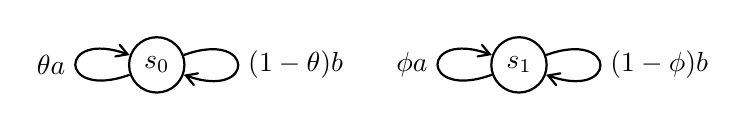
\begin{tikzpicture}[scale=2.3,LMC style]
	\node[state] (s0) at (-1,0) {$s_0$};
	\node[state] (s1) at (1,0) {$s_1$};
	
	\path[->] (s0) edge [loop,out=200,in=160,looseness=10] node[pos=0.5,left] {$\theta a$} (s0);
	\path[->] (s0) edge [loop,out=20,in=340,looseness=10] node[pos=0.5,right] {$(1 - \theta) b$} (s0);
	\path[->] (s1) edge [loop,out=200,in=160,looseness=10] node[pos=0.5,left] {$\phi a$} (s1);
	\path[->] (s1) edge [loop,out=20,in=340,looseness=10] node[pos=0.5,right] {$(1 - \phi) b$} (s1);
	\end{tikzpicture}
\end{center}

By (INSERT THM) we may compute $\lim_{n \rightarrow \infty} \frac{1}{n} \ln L_n$ to be
\begin{equation*}
\phi \ln \theta + (1 - \phi) \ln (1 - \theta))  - \phi \ln \phi -  (1 - \phi) \ln (1 - \phi))
\end{equation*}
Suppose $w \in \Sigma^n$ contains $k$ instances of the letter $a$, then
$\PP_{s_0} (w) = \theta^{k} (1 - \theta)^{n - k}$ and $\PP_{s_1} (w) = \phi^{k} (1 - \phi)^{n - k}$ it follows that

\begin{align*}
\PP_{s_0}(w) \leq \PP_{s_1}(w) & \iff \theta^{k} (1 - \theta)^{n - k} \leq \phi^{k} (1 - \phi)^{n - k} \\
& \iff \Big( \frac{\theta (1 - \phi)}{\phi (1 - \theta)} \Big)^k \leq \Big( \frac{1 - \phi}{1 - \theta}\Big)^n \\
& \iff k \leq n ~\frac{\ln \frac{1 - \phi}{1 - \theta}}{\ln\frac{\theta(1 - \phi)}{\phi(1 - \theta)}} \\
\end{align*}

Let $\gamma = \frac{\ln \frac{1 - \phi}{1 - \theta}}{\ln\frac{\theta(1 - \phi)}{\phi(1 - \theta)}}$, then using the inequalities $1 - \frac{1}{x} \leq \ln x \leq x - 1$ it follows that 

\begin{equation*}
\gamma  = \frac{1}{1 + \ln \frac{\theta}{\phi} / \ln \frac{1 - \phi}{1 - \theta}} \leq \frac{1}{1 + (1 - \frac{\phi}{\theta})/ (\frac{1 - \phi}{1 - \theta} - 1)} = \frac{\frac{1 - \phi}{1 - \theta} -  1}{\frac{1 - \phi}{1 - \theta} - \frac{\phi}{\theta}} = \theta \frac{\theta - \phi}{\theta - \phi \theta - \phi + \phi\theta} = \theta.
\end{equation*}
Similarly $\phi \leq \gamma$.

The function $s \rightarrow \theta^s(1 - \theta)^{n - s}$ which by considering its derivative is increasing for $0 \leq s \leq \theta n$. Similarly, $s \rightarrow \phi^s(1 - \phi)^{n - s}$ is decreasing for $\phi n \leq s \leq n$.


\begin{align*}
\lim_{n \rightarrow \infty} \Big(\sum_{w \in \Sigma^n} \text{min}(w) \Big)^\frac{1}{n} & = \lim_{n \rightarrow \infty} \Big( \sum_{k = 0}^{\floor*{\gamma n}} {n \choose k} \theta^k(1 - \theta)^{n - k} + \sum_{k = \floor*{\gamma n}+1}^{n} {n \choose k} \phi^k(1 - \phi)^{n - k} \Big)^{\frac{1}{n}} \\
& = \frac{ \max \{ \theta^\gamma (1 - \theta)^{1- \gamma}, \phi^\gamma (1 - \phi)^{1- \gamma}\}}{\gamma^\gamma (1 - \gamma)^{1 - \gamma}}
\end{align*}

\section{Computing Likelihood Exponents}\label{seccompdet}

We first discuss the convergence properties of $\liexp$. We say a set of states in an HMM $S \subseteq Q$ is \emph{irreducible} if for all $i,j \in S$, there exists a word $w \in \Sigma^*$ such that $\Psi(w)_{i,j} > 0$. An HMM is irreducible if $Q$ is irreducible. An irreducible HMM is \emph{mortal} if for some word $w \in \Sigma^*$, $\Psi(w) = 0$. 

Consider a discrete probability measure $r : \Sigma \rightarrow [0,1]$. We may construct a single state HMM $(q, \Sigma, \Psi_{\text{ind}})$ that produces a sequence of independent letters sampled from the distribution given by $r$ by letting $\Psi_{\text{ind}}(a) = r(a)$.

Now consider the union of this HMM with an irreducible HMM $(Q, \Sigma, \Psi)$ with the same set of observations. The union has states $Q \cup \{q\}$, observations $\Sigma$ and observation density matrix defined in blocks as 
\begin{equation}
\overline{\Psi}(a)  = \begin{pmatrix}
\Psi(a) && 0\\
0  && \Psi_{\text{ind}}(a)\\
\end{pmatrix}.
\end{equation}
For arbitrary initial distribution $\pi_1$ and $\pi_2 = \delta_q$ fixed, convergence of $\liexp$ is a consequence of \cite{prot13}. We write $\PPind$ for the probability measure on $\Sigma^\omega$ corresponding to words produced starting from $\pi_2$. A version of the main theorem is stated below.

\begin{theorem}\textsc{\textbf{Protasov's Theorem}}
Let $\pi_1$ be an initial distribution. If an irreducible HMM $(Q, \Sigma, \Psi)$ is mortal, then $\lyapexp = -\infty \quad \PPind$-a.s. otherwise there is a $\lambda \in (-\infty, 0]$ such that $\lyapexp = \lambda \quad \PPind$-a.s.
\end{theorem}
Since, $\liexp = \lyapexp - \lim_{n \rightarrow \infty} \frac1n \ln \pi_2 \Psi_n \1^T$, in this case convergence of $\liexp$ follows from Protasov's Theorem. When the HMM is not irreducible, we may generalise this theorem as follows

In the next section we show how to reduce the general case to this one.

\subsection{Cross Product Construction}

When the probability space on infinite words is derived from a general HMM, the probability of a particular letter being produced at a specific position in the infinite word depends on the state that the HMM is in. To overcome this issue, we build a \emph{cross-product cocycle} where current state of the producing HMM as started from $\pi_2$ is incorporated into the state space of the HMM started from $\pi_1$. 

To accomplish this, we simulate transitions in the producing HMM by sampling a uniform random number in the interval $[0,1)$. At each state, we may partition $[0,1)$ so that each sub-interval corresponds to specific transition and the size of the sub-interval corresponds to the probability of said transition. The union over all states of these partitions has a minimal finite $\sigma$-algebra. The atoms of this $\sigma$-algebra are also a partition of $[0,1)$ and so we may sample them independently at random with probabilities according to their size. The transformation is demonstrated in the diagram below.

\begin{center}
	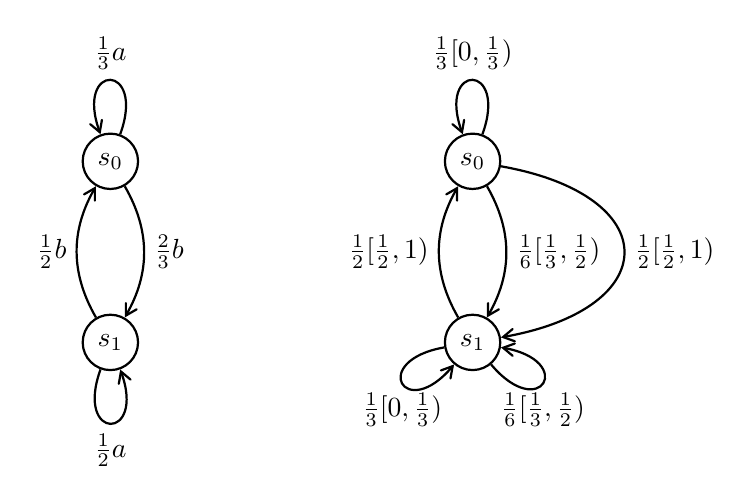
\begin{tikzpicture}[scale=2.3,LMC style]
	\node[state] (s0) at (-1,1) {$s_0$};
	\node[state] (s1) at (-1,0) {$s_1$};
	\node[state] (s2) at (1,1) {$s_0$};
	\node[state] (s3) at (1,0) {$s_1$};

	
	\path[->] (s0) edge [loop,out=70,in=110,looseness=10] node[pos=0.5,above] {$\frac13 a$} (s0);
	\path[->] (s1) edge [loop,out=250,in=290,looseness=10] node[pos=0.5,below] {$\frac12 a$} (s1);
	\path[->] (s1) edge[bend left] node[left,pos=0.5] {$\frac12 b$} (s0);
	\path[->] (s0) edge[bend left] node[right,pos=0.5] {$\frac23 b$} (s1);
	
	
	\path[->] (s2) edge [loop,out=70,in=110,looseness=10] node[pos=0.5,above] {$\frac13 [0,\frac13)$} (s2);
	\path[->] (s3) edge [loop,out=190,in=230,looseness=10] node[pos=0.5,below] {$\frac13 [0,\frac13)$} (s3);
	\path[->] (s3) edge [loop,out=310,in=350,looseness=10] node[pos=0.5,below] {$\frac16 [\frac13,\frac12)$} (s3);
	
	\path[->] (s3) edge[bend left] node[left,pos=0.5] {$\frac12 [\frac12, 1)$} (s2);
	\path[->] (s2) edge[bend left] node[right,pos=0.5] {$\frac16 [\frac13,\frac12)$} (s3);
	\path[->] (s2) edge[bend left, out=80, in=100, looseness = 2.5] node[right,pos=0.5] {$\frac12 [\frac12, 1)$} (s3);
	
	\end{tikzpicture}
\end{center}

Consider the HMM $(Q, \Sigma, \Psi)$ with finite alphabet $\Sigma$. Since for each $i \in [Q]$, $\sum_{a \in \Sigma} \sum_{j = 1}^{|Q|} \Psi(a)_{i,j} = 1$ it follows that we may define a function $\rho_i : [0,1) \rightarrow Q \times \Sigma$ such that for all $i \in [Q]$, $\MLeb(\rho_i^{-1}\{(j, a)\}) = \Psi(a)_{i,j}$. Consider the minimal $\sigma$-algebra $\sigma\{\rho_i^{-1}\{(j, a)\} \mid i,j \in [Q], a \in \Sigma\}$ which is finite and has a set of atomic elements $P$ of at most $|Q|^2|\Sigma|$ elements. $P$ is also a partition of $[0,1)$. Let $p \in P$ then $\rho_i(x)$ is constant for all $x \in p$ so we may overload the notation and consider the function $\rho_i : P \rightarrow Q \times \Sigma$. 

We will describe the one-state chain $(\{1\}, P, \Psi_P)$ as the \emph{singleton generator} for $\Psi$ where $\Psi_P(p) = \MLeb(p)$. Given an initial distribution $\pi$ for $(Q, \Sigma, \Psi)$, a word generated by its singleton generator uniquely defines a path of states and letters. Let $\PPind$ be the measure on the set of infinite words $P^\omega$ generated by this HMM.

In order to incorporate the state space of the producing HMM into the state space of the chain started from $\pi_1$, we define two functions $l : Q \times \Sigma \rightarrow Q$ and $r : Q \times \Sigma \rightarrow \Sigma$ where $l(q,a) = q$ and $r(q,a) = a$. We then define the cross-product cocycle $\Psi^* : P \rightarrow [0,1]^{(Q \times Q) \times (Q \times Q)}$ as 
\[\Psi^*(p)_{(i_1,j_1),(i_2,j_2)} = \begin{cases} 
\Psi(r \circ \rho_{j_1}(p) )_{i_1, i_2} & l \circ \rho_{j_1}(p) = j_2 \\
0 & \text{else}. \\
\end{cases}\]

We may extend $\Psi^*$ in the usual way to $P^n$ and write $\Psi_n^*$ for the associated random variable on $P^n$ under measure $\PPind$. This leads to the following Theorem.

\begin{theorem}
Consider the HMM $(Q, \Sigma, \Psi)$ with initial distributions $\pi_1$ and $\pi_2$ then for any measurable set $A \in [-\infty, 0]$
\begin{equation*}
\PP_{\pi_2}\big( \lim_{n\rightarrow\infty} \frac1n \ln L_n \in A\big) = \PPind\big(\lim_{n\rightarrow\infty} \frac1n \ln \frac{\pi_1 \times \pi_2 \Psi^* \1}{\pi_2 \times \pi_2 \Psi^* \1} \in A \big).
\end{equation*}
In addition, the random variable $\lim_{n\rightarrow\infty} \frac1n \ln L_n$ takes at most $|Q|^2$ values with non-zero probability under the $\PPind$ measure.
\end{theorem}

We will write $\Epsilon_{\pi_1, \pi_2}$ for the set of values attained by $\liexp$ with $\PPind$ non-zero probability. 

\begin{corollary}\label{subcompcalc}
Let $(Q, \Sigma, \Psi)$ then we may produce $K \leq |Q|^2$ irreducible cocycles $\Psi_k$ and pairs of initial distributions $(a_1, b_1) \dots, (a_K, b_K)$ in time $O(|Q|^4|\Sigma|)$ such that $\lim_{n \rightarrow \infty} \frac1n \ln L_n^{a_k, b_k}$ converges to a constant $\PP_{b_k}$-almost surely and
\begin{equation*}
\Epsilon_{\pi_1, \pi_2} \subseteq \bigcup_{k = 1}^K \Epsilon_{a_k, b_k}.
\end{equation*}
\end{corollary}

\end{example}

\begin{example}\label{twostateex}
Let $1 > \theta > \phi \geq \frac12$ and consider the disconnected HMM
\begin{center}
	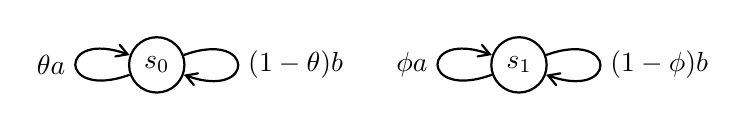
\begin{tikzpicture}[scale=2.3,LMC style]
	\node[state] (s0) at (-1,0) {$s_0$};
	\node[state] (s1) at (1,0) {$s_1$};
	
	\path[->] (s0) edge [loop,out=200,in=160,looseness=10] node[pos=0.5,left] {$\theta a$} (s0);
	\path[->] (s0) edge [loop,out=20,in=340,looseness=10] node[pos=0.5,right] {$(1 - \theta) b$} (s0);
	\path[->] (s1) edge [loop,out=200,in=160,looseness=10] node[pos=0.5,left] {$\phi a$} (s1);
	\path[->] (s1) edge [loop,out=20,in=340,looseness=10] node[pos=0.5,right] {$(1 - \phi) b$} (s1);
	\end{tikzpicture}.
\end{center}
Starting the chain from $s_1$ leads to an independent production of letters. Additionally in this case, the expressions $e_{s_0}\Psi(w)\1^T$ can be written as $\theta^k (1 - \theta)^{n - k}$ where $k$ is the number of observations labelled $a$ in $w$. Similarly, the likelihood ratio $L_n(w) = \Big(\frac{\theta}{\phi}\Big)^k \Big(\frac{1 - \theta}{1 - \phi}\Big)^{n-k}$ and so 
\begin{equation*}
\frac1n \ln L_n = \frac{k}{n}\ln\frac{\theta}{\phi} + \frac{n - k}{n}\ln\frac{1 - \theta}{1- \phi} \rightarrow \phi \ln\frac{\theta}{\phi} + (1 - \phi) \ln\frac{1 - \theta}{1- \phi} 
\end{equation*}
as $n \rightarrow \infty$ since the ratio $k/n$ tends to $\phi$ almost surely.  Therefore the likelihood exponent is symbolically computable. 
\end{example}

\begin{lemma}
Suppose that $\PP_{\pi_1}(L_n < 1) - \PP_{\pi_2}(L_n < 1) \geq 1 - e^{An + B}$ for some $A, B \in \RR$. Then
\begin{equation*}
\liexp \leq A \quad \pi_2\text{-a.s.}
\end{equation*}
\end{lemma}

\begin{proof}
Fix $A < \alpha < 0$ and define the event $W_n = \{1 > L_n \geq \e^{n\alpha}\}$. Then
\begin{align*}
\PP_{\pi_2}(\lim_{n \rightarrow \infty} \frac1n \ln L_n > \alpha) & \leq \PP_{\pi_2}(\liminf_n \{\frac1n \ln L_n \geq \alpha\}) \\
& \leq \liminf_n \PP_{\pi_2}(\frac1n \ln L_n \geq \alpha) \\
& \leq \liminf_n \PP_{\pi_2}(L_n \geq \e^{n\alpha}) \\
& = \liminf_n \Big[ \PP_{\pi_2}(1 > L_n \geq \e^{n\alpha}) +  \PP_{\pi_2}(L_n \geq 1) \Big]\\
& \leq \liminf_n \Big[ \sum_{w \in W_n} \pi_2 \Psi(w) \1^T + e^{An + B} \Big]\\
& \leq \liminf_n \Big[ e^{-n\alpha} \sum_{w \in W_n} \pi_1 \Psi(w) \1^T\Big]\\
& \leq \liminf_n \Big[ e^{-n\alpha} \PP_{\pi_1}(L_n < 1)\Big]\\
& \leq \liminf_n \Big[ e^{-n\alpha} e^{An + B}\Big]\\
& = 0.
\end{align*}
\end{proof}
Now suppose $\pi_1$ and $\pi_2$ are distinguishable.  By Theorem 5 of \cite{kief16} one may compute a $c \in (-\infty, 0)$ such that 
\begin{align*}
\PP_{\pi_1}(L_n < 1) - \PP_{\pi_2}(L_n < 1) & \geq 1 - 2e^{cn} \\
& \geq 1 - 2e^{n \max\Lambda }
\end{align*}

For a given HMM $(Q, \Sigma, \Psi)$, we may define a \emph{monitor} as a function $M_n : \Sigma^n \rightarrow \{1,2\}$. A well designed monitor reads an input word from an HMM started with either $\pi_1$ or $\pi_2$ and aims to return $1$ or $2$ respectively with high probability. However the following series of inequalities hold

\begin{align*}
\PP_{\pi_2}(M_n(w) = 2) - \PP_{\pi_1}(M_n(w) = 2)  &= \PP_{\pi_2}(M_n(w) = 1) + \PP_{\pi_1}(M_n(w) = 2) \\
& = \sum_{w \in \Sigma^n} \pi_1 \Psi(w) \1^T \delta_{M_n(w) = 1} + \pi_2 \Psi(w) \1^T \delta_{M_n(w) = 2} \\
& \geq \sum_{w \in \Sigma^n} \pi_1\Psi(w)\1^T \land \pi_2 \Psi(w) \1^T \\
& = \PP_{\pi_2}(L_n \leq 1) - \PP_{\pi_1}(L_n \leq 1)
\end{align*}
which means for any monitor, to guarantee an error probability bound of at most $\epsilon$, we require atleast $\frac{\ln(\epsilon) - \ln 2}{\max \Lambda}$ observations. This bound motivates us to investigate computability properties of $\Lambda$. 


\end{document}
  